\chapter{Experiments and results}
\label{ch:exp}

\section{Gradient peak}\label{sec:gradient-peak}
As stated before, the input perturbation, output-correlation method in~\cite{Hammer-2021} did not point to high-gamma frequency amplitude as being strikingly important to the network. The gradient visualization also did not show particularly high gradients in the high-gamma band, unless the input window for the network was shortened so that the network had only one output, i.e. predicted one time-point. Two interesting observations could be made for the one-output gradient visualization:
\begin{itemize}
\item[1.] A gradient peak occurs at 83.88 Hz in both the untrained and the trained network and it is amplified with training.
\item[2.] If we add noise of a certain frequency or white noise to the input, frequencies around 83.33 Hz increases in the output of the network.
\end{itemize}

83.33Hz seems like a random frequency to have such a sharp peak in the frequency and also does not seem to be caused by a physiological property of the input signal.
A hypothesis was that the 83.33 Hz peak occurs due to this frequency being aligned with the dilations of the max-pool layers and therefore is just an architecture artifact.
Because sampling rate is 250 Hz and the dilations of the max-pool layers are powers of three and $250 Hz / 3 = 83.33 Hz$, this frequency aligns with the dilations of the max-pool layers which amplify it.
However, this does not explain why the peak at 83.33Hz is amplified with training.

To test the artifact hypothesis, we systematically changed the dilations of the max-pool layers to powers of 1, 2 and 3 and kernel sizes to 1\footnote{Importantly, when all max-pool layers in a network have their kernel size set to 1, it is equivalent to a network without max-pool layers.}, 2, 3 and 4

The results in Figure~\ref{fig:gradient-peak} demonstrate that the kernel size change has no effect on the 83.33Hz peak.
However, with change in the dilations, the 83.33 Hz peak disappears without a decrease in performance.
Another interesting thing to notice is to observe how the gradients of motor, non-motor and all channels behave with respect to each other.
The biggest differences between the gradients are in the alpha and beta bend where the motor gradients have visibly higher values than non-motor and all channels.
For the gradient peak at 83.33 Hz, the values of the motor, non-motor and all channels are almost equivalent.

\begin{figure}
\begin{subfigure}{.5\textwidth}
  \centering
  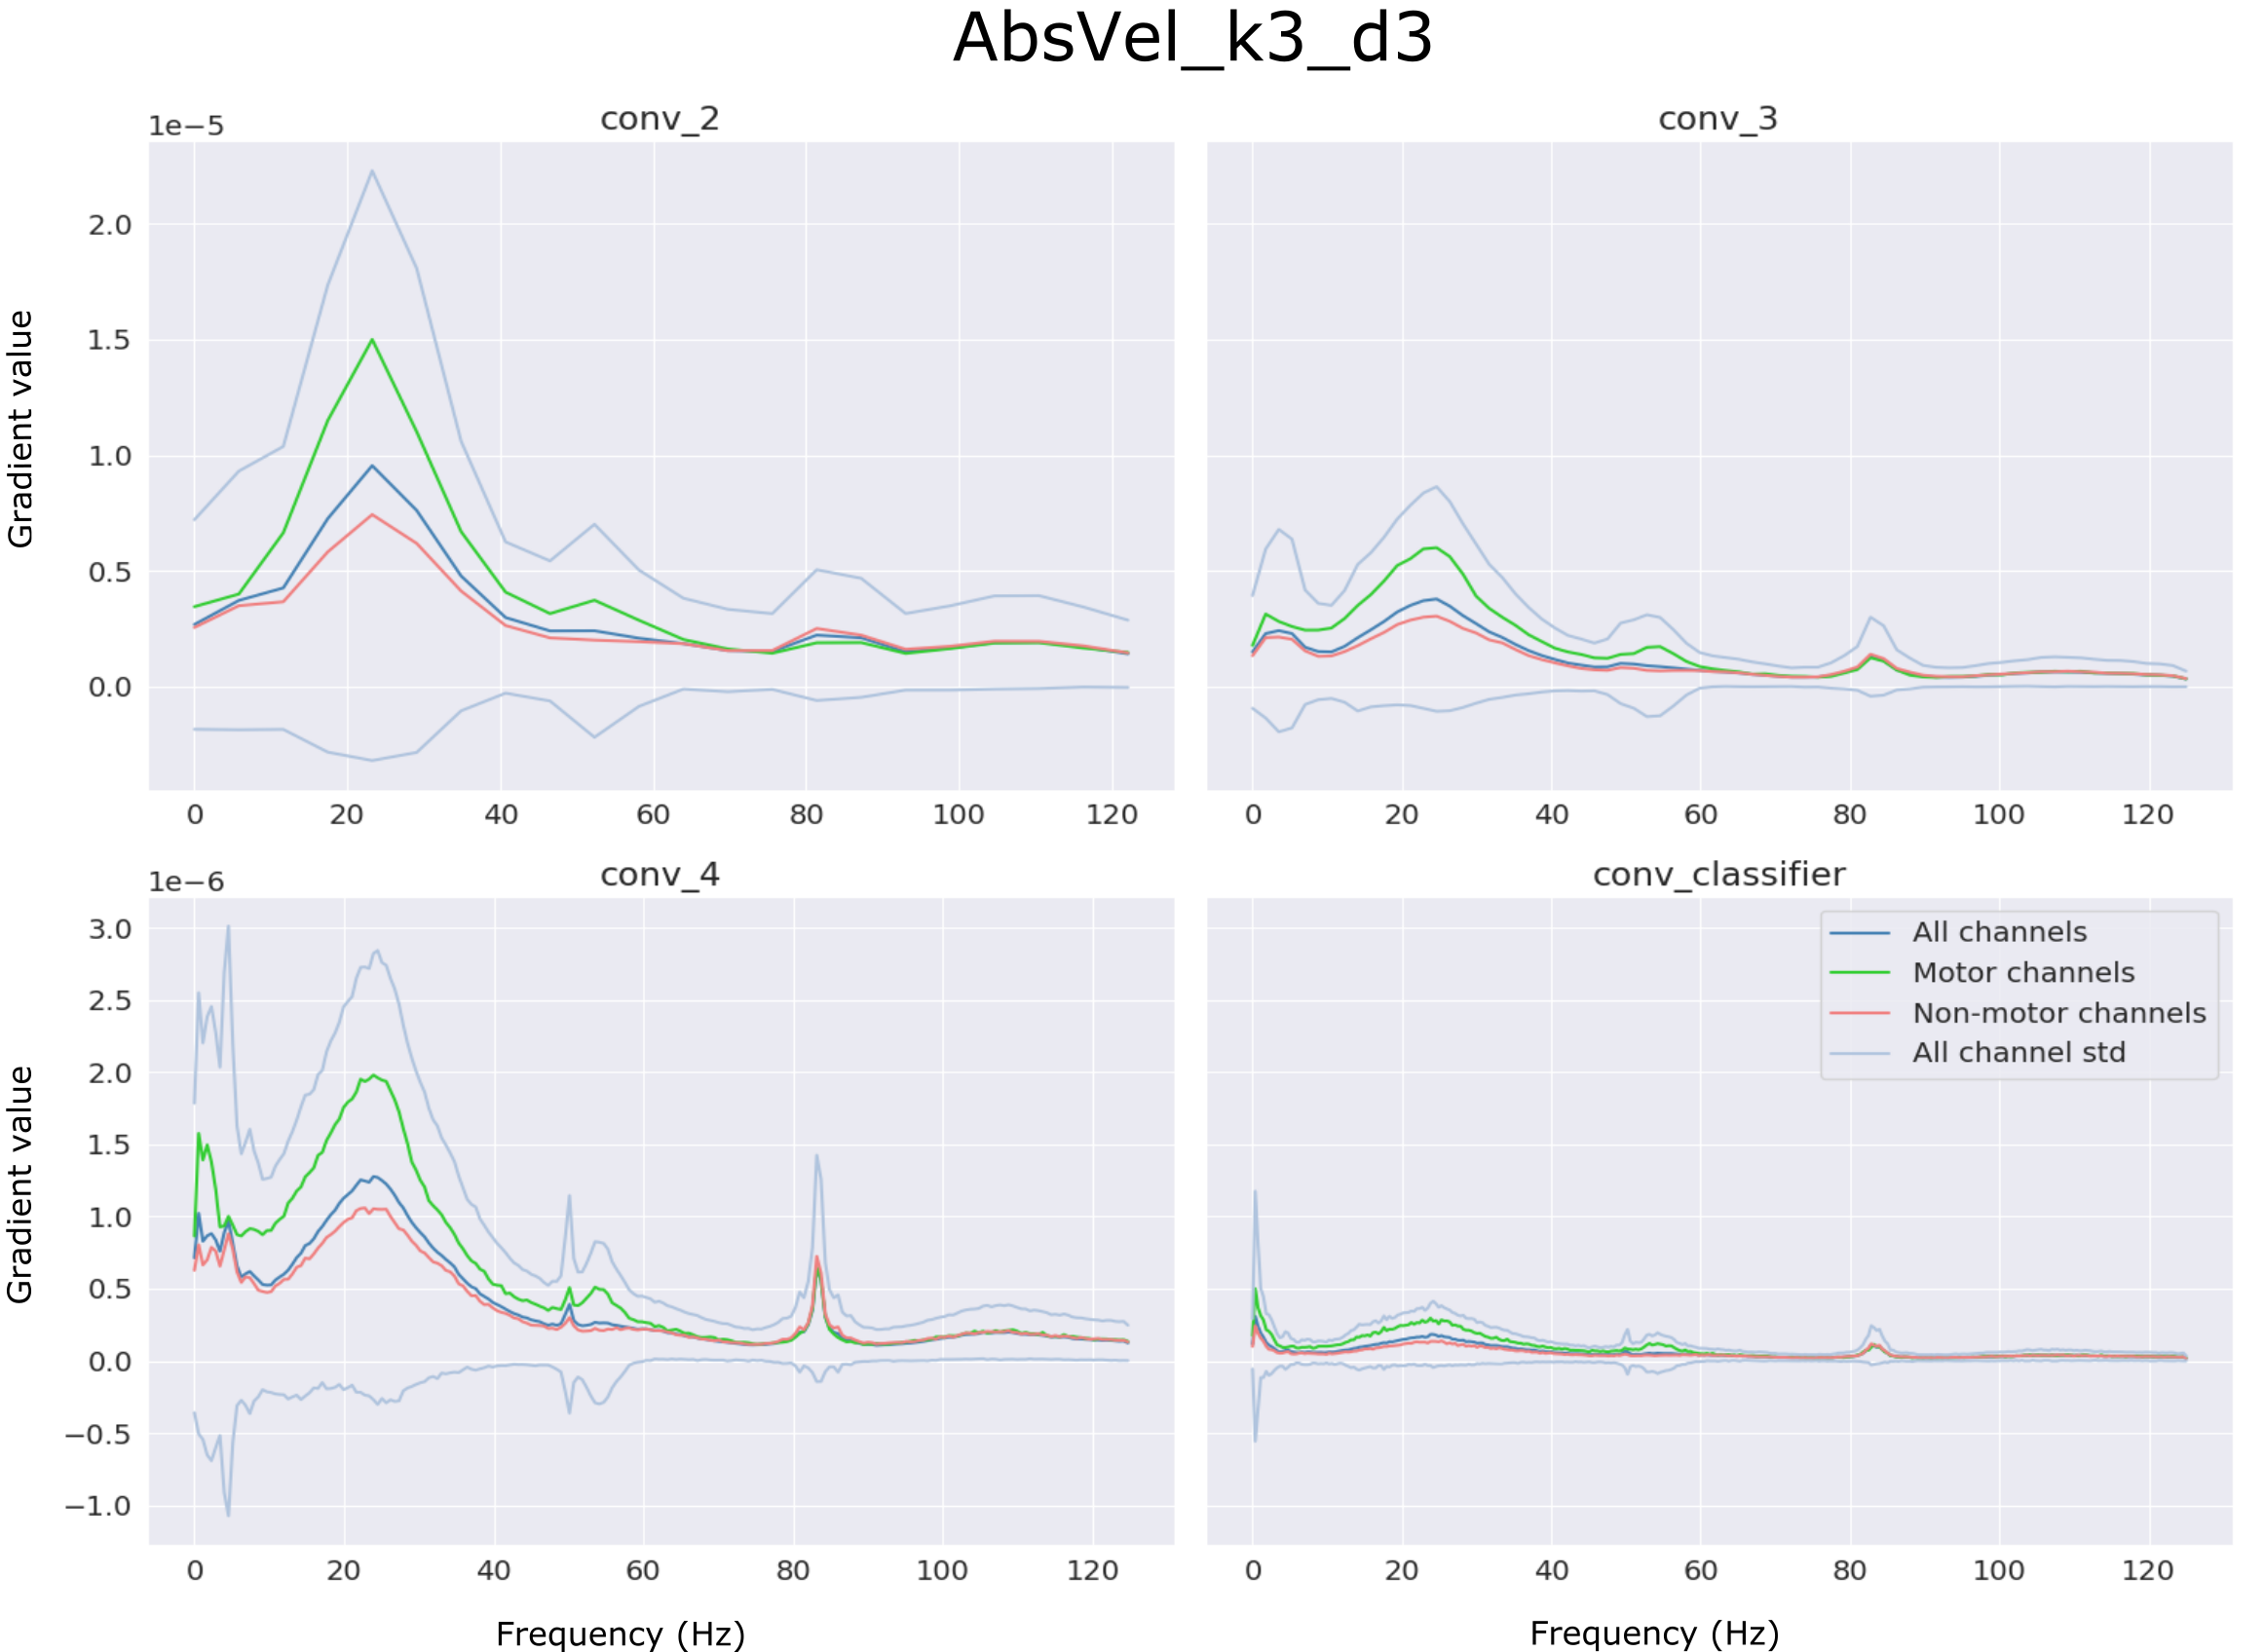
\includegraphics[width=.8\linewidth]{img/ch4/absVel-k3-d3}
  \caption{1a}
  \label{fig:absVel-k3-d3}
\end{subfigure}%
\begin{subfigure}{.5\textwidth}
  \centering
  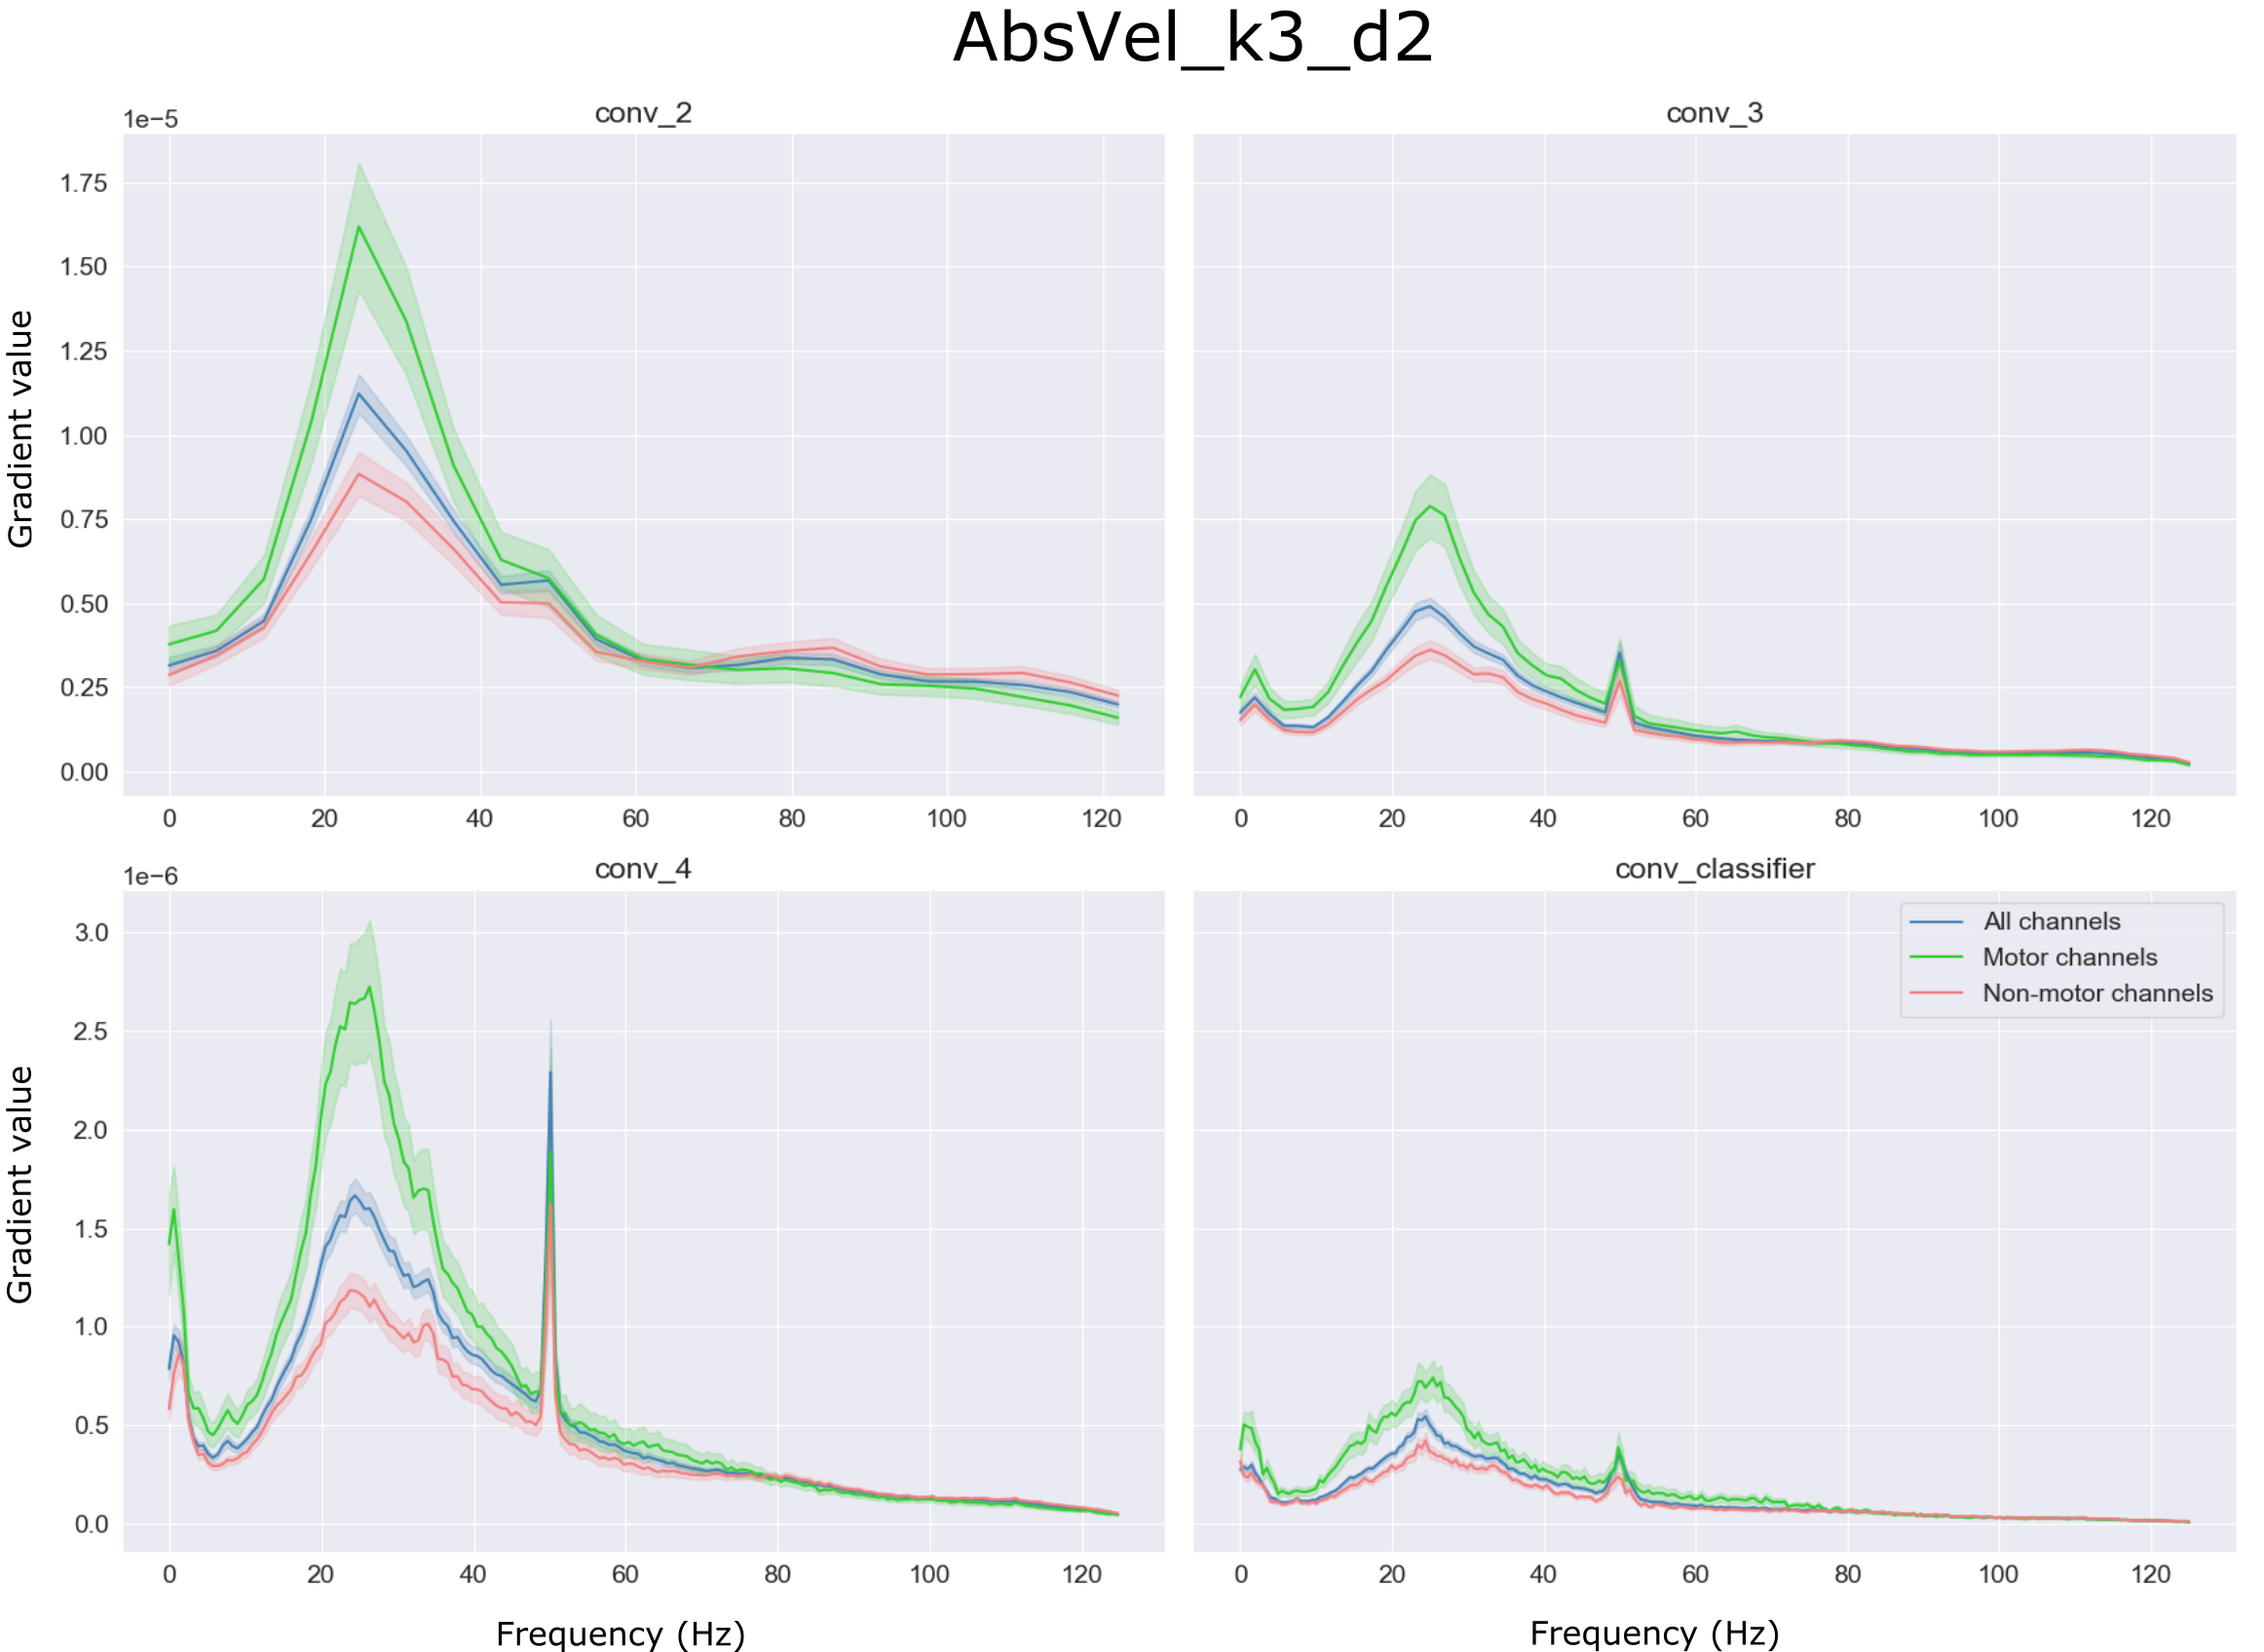
\includegraphics[width=.8\linewidth]{img/ch4/absVel-k3-d2}
  \caption{1b}
  \label{fig:absVel-k3-d2}
\end{subfigure}
\begin{subfigure}{.5\textwidth}
  \centering
  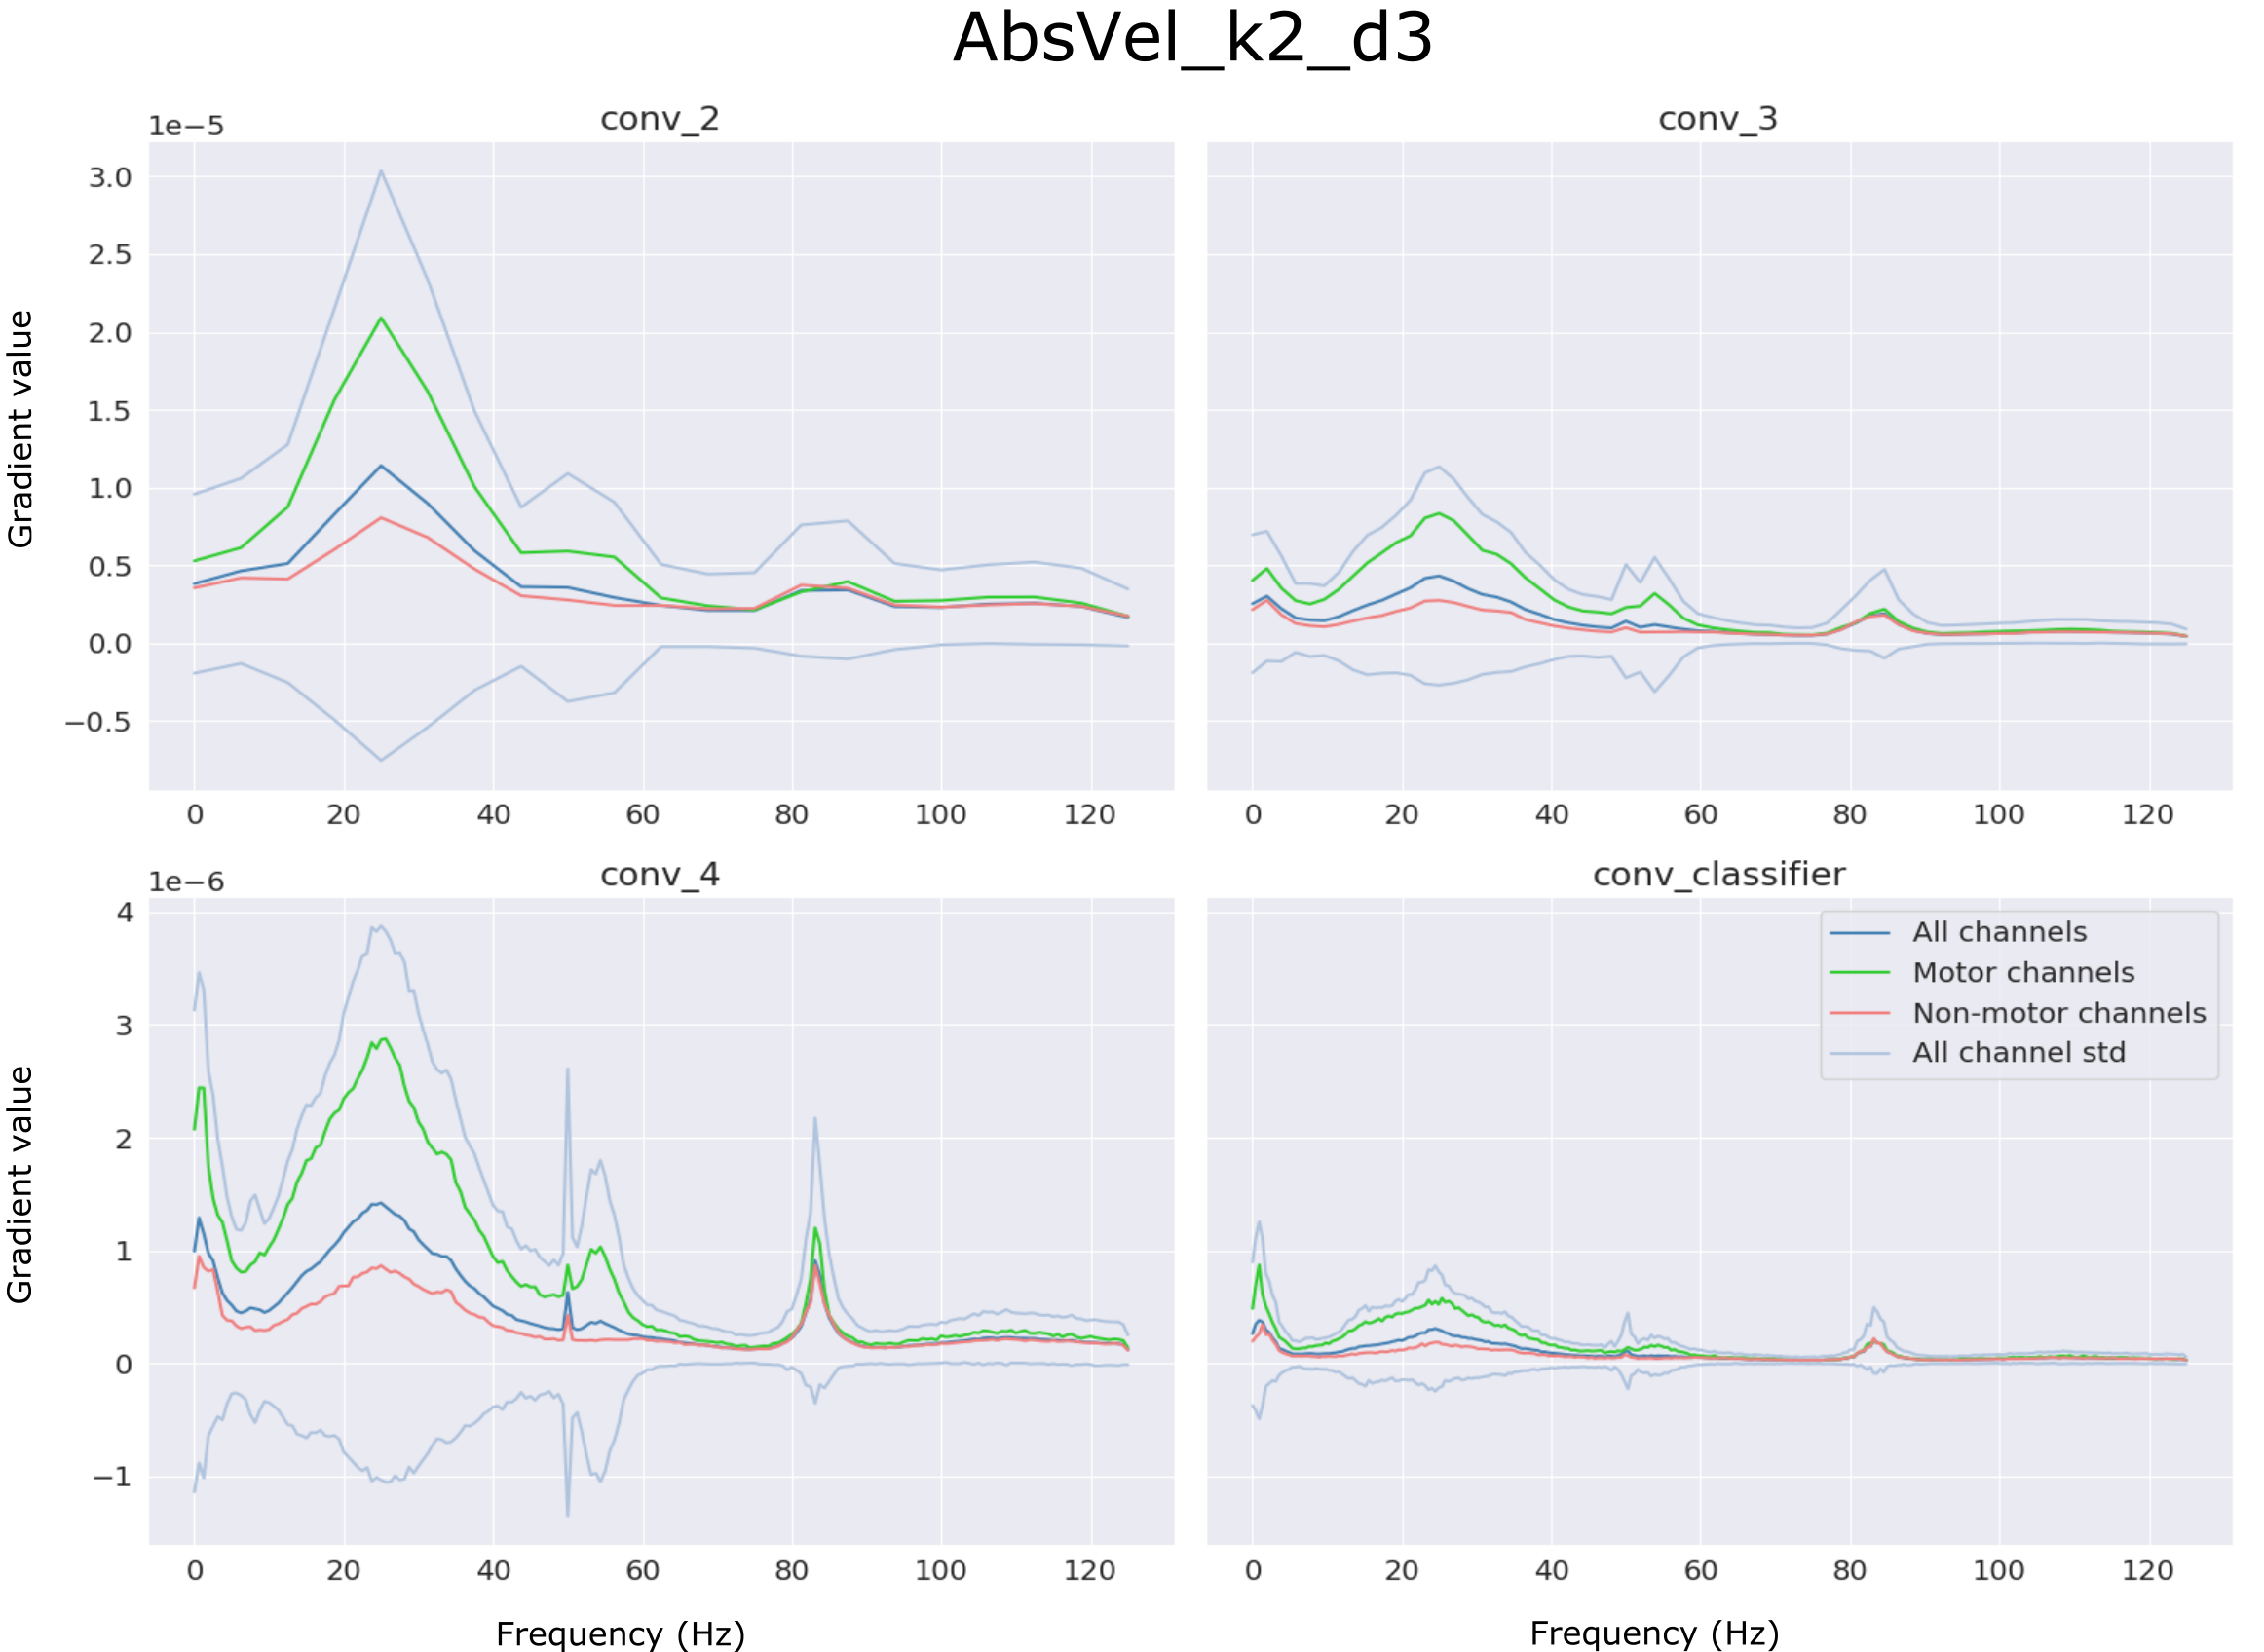
\includegraphics[width=.8\linewidth]{img/ch4/absVel-k2-d3}
  \caption{1a}
  \label{fig:absVel-k2-d3}
\end{subfigure}%
\begin{subfigure}{.5\textwidth}
  \centering
  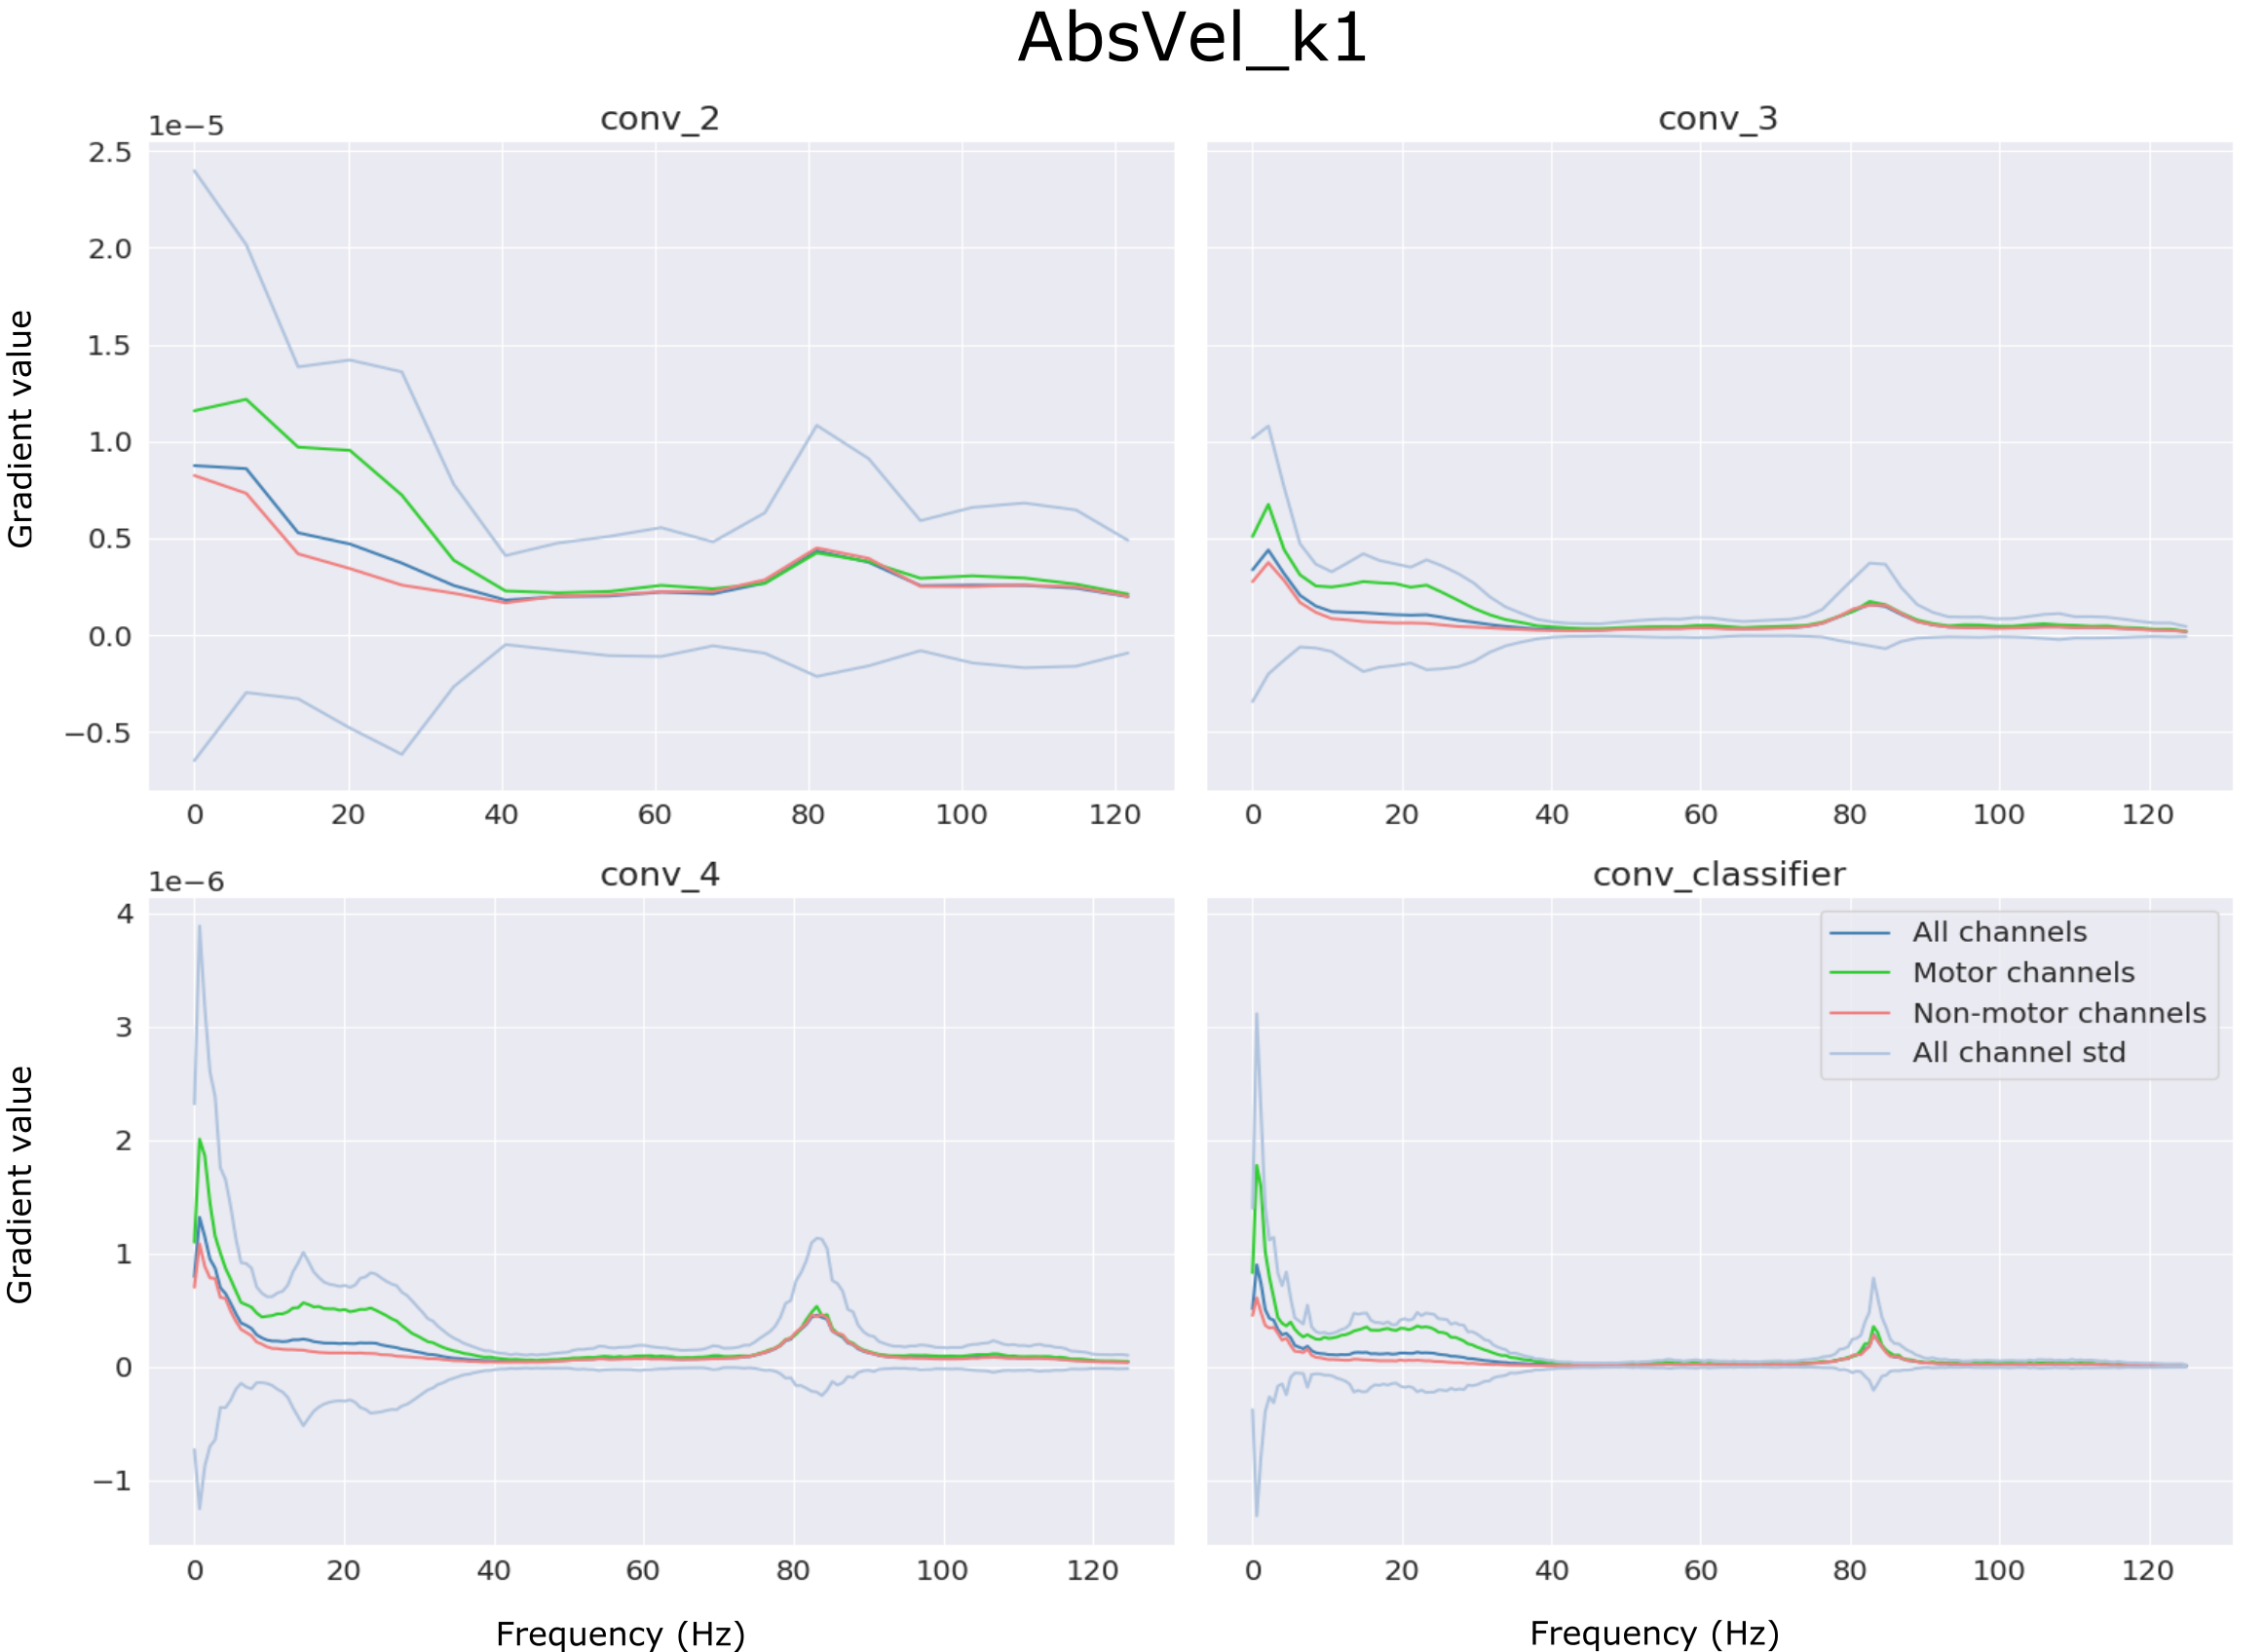
\includegraphics[width=.8\linewidth]{img/ch4/absVel-k1}
  \caption{1b}
  \label{fig:absVel-k1}
\end{subfigure}
\caption{plots of....}
\label{fig:gradient-peak}
\end{figure}

We also studied how the signal is affected by max-pool layers only.
We used one and three max-pool layers with dilations equivalent with those from the Deep4Net.
When the max-pool layer dilation parameter was three (or powers of three in the case of multiple consecutive max-pool layers), the output signal exhibited periodical peaks with the greatest peak around 83.33Hz.
When the dilation of the max-pool layers shifted to two and powers of two, the periodicity of the peaks still occurred, however, the period increased and the greatest peak was around 120Hz.
This is in line with the hypothesis that the alignment of frequencies with the max-pool layer dilations is indeed the reason for the gradient peak we see in Figure~\ref{fig:max-pool-changes}.

%\begin{figure}
%\begin{subfigure}{1\textwidth}
%  \centering
%  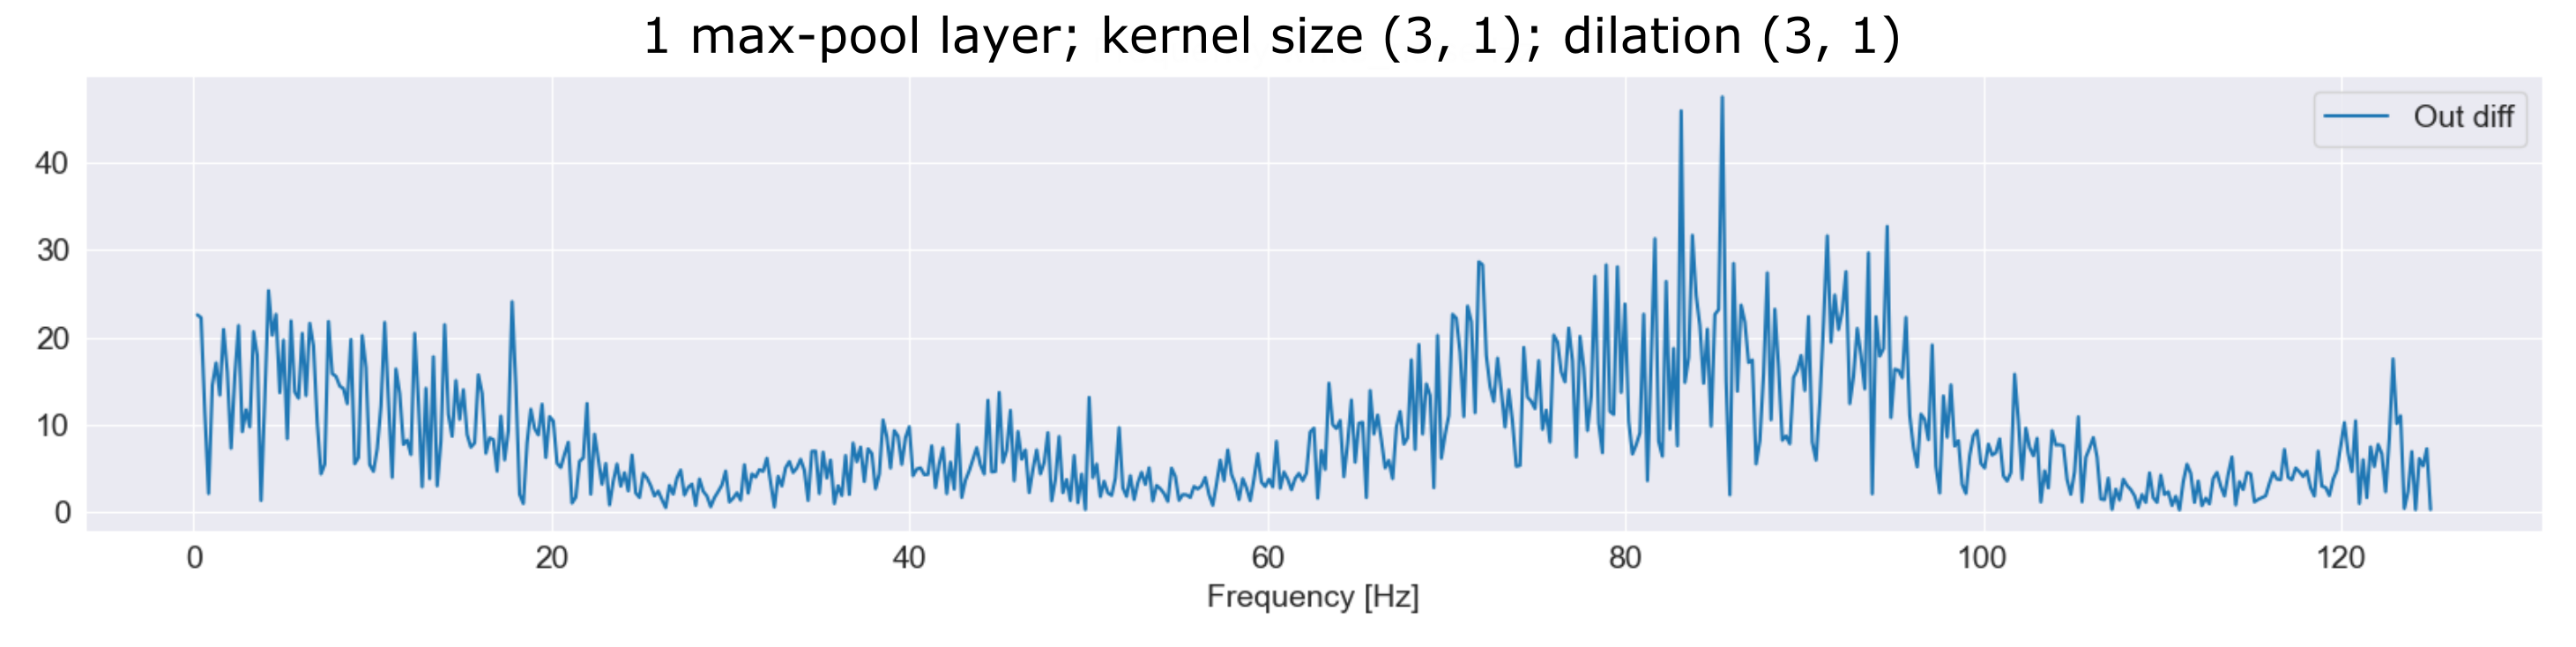
\includegraphics[width=1\linewidth]{img/ch4/absVel-maxpool-k3-d3}
%%  \caption{1a}
%  \label{fig:maxpool-k3-d3}
%\end{subfigure}%
%\begin{subfigure}{1\textwidth}
%  \centering
%  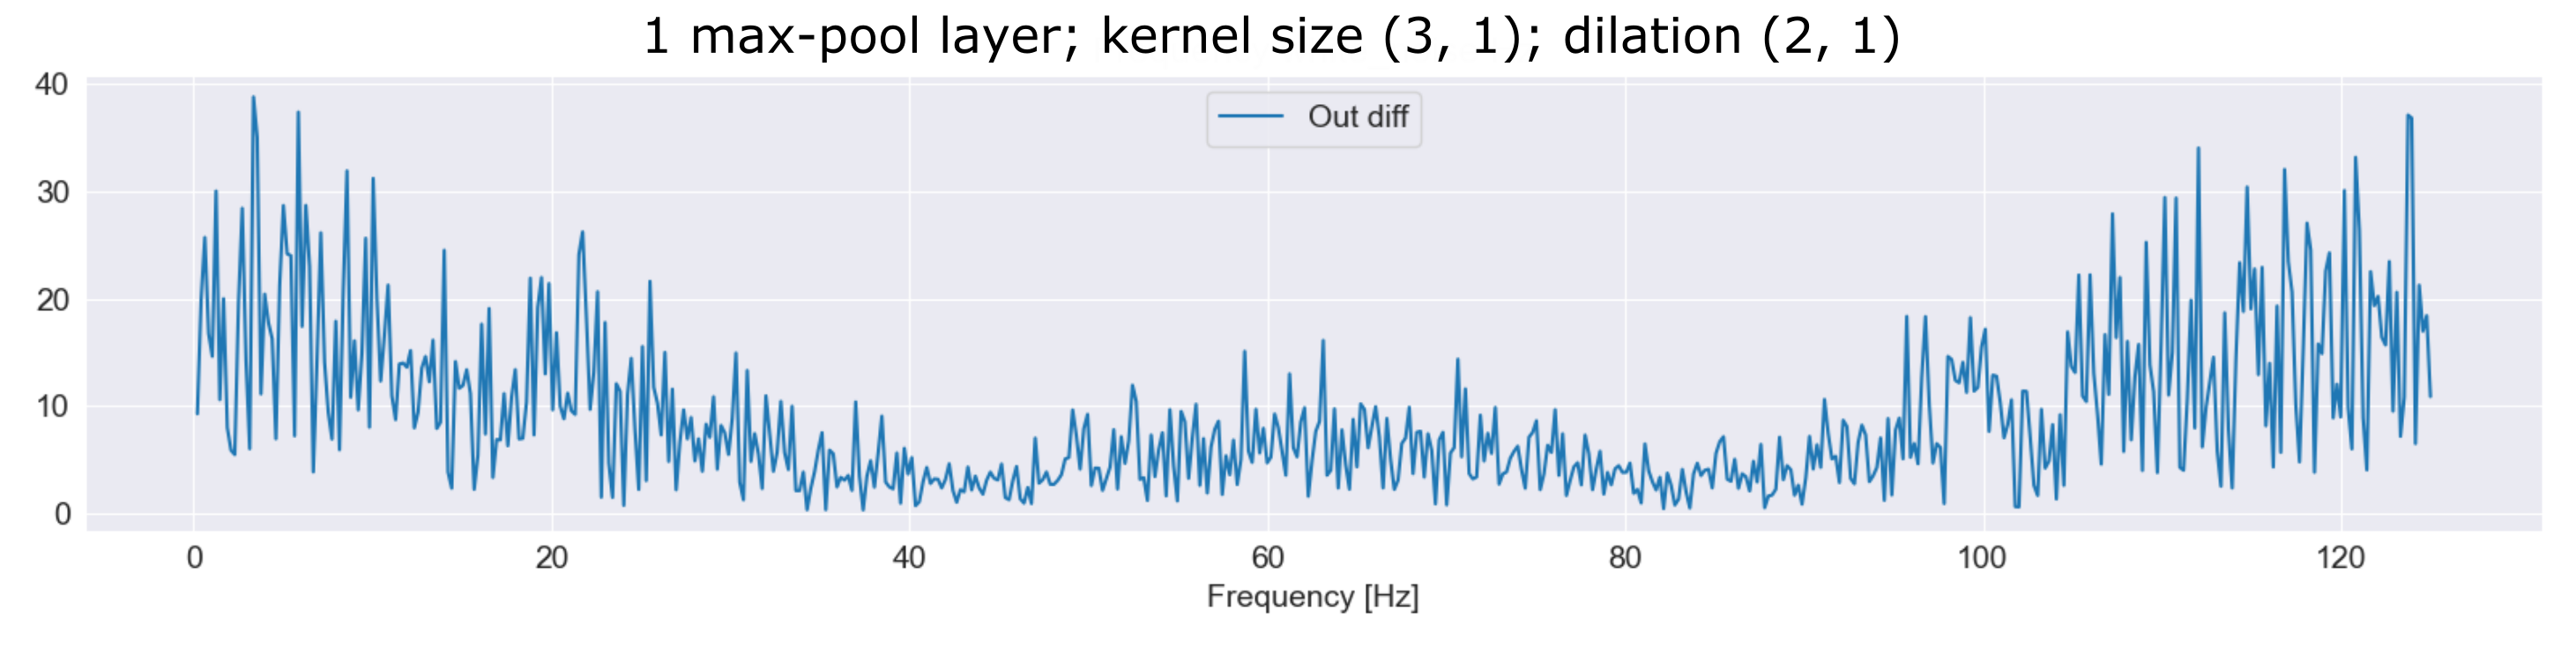
\includegraphics[width=1\linewidth]{img/ch4/absVel-maxpool-k3-d2}
%  \caption{1b}
%  \label{fig:maxpool-k3-d2}
%\end{subfigure}
%\caption{plots of....}
%\label{fig:max-pool-changes}
%\end{figure}%%

\begin{figure}
\centering
\begin{subfigure}[b]{\textwidth}
   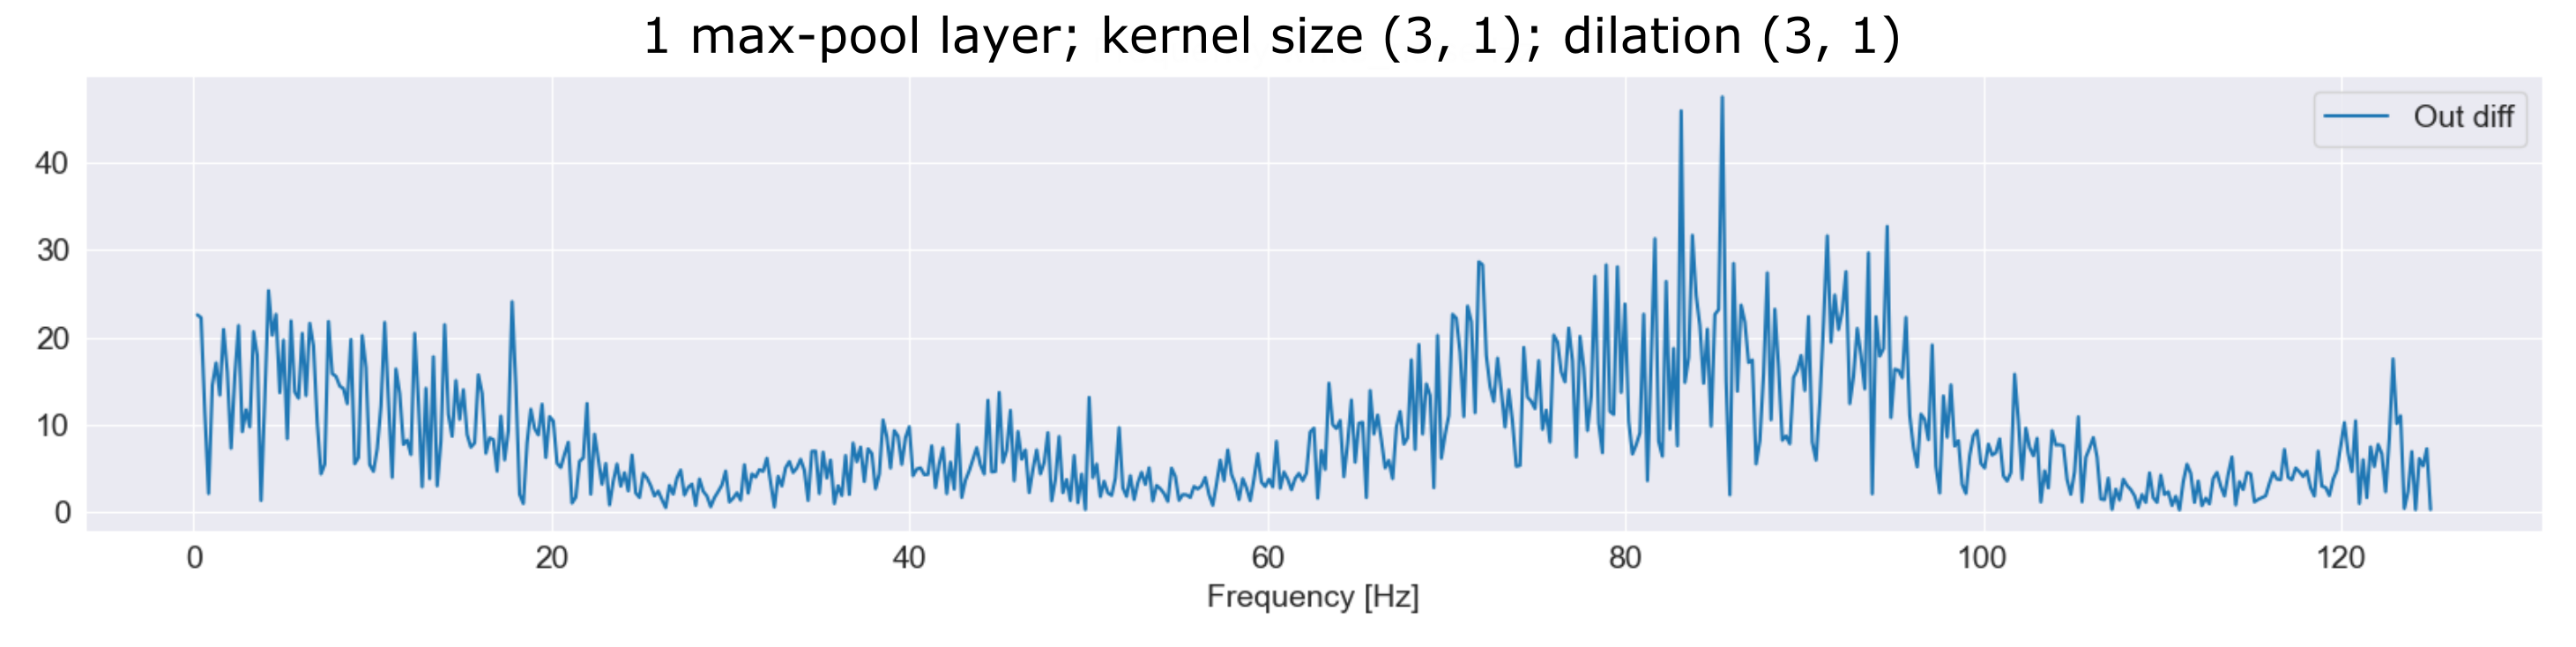
\includegraphics[width=1\linewidth]{img/ch4/absVel-maxpool-k3-d3}
   \caption{}
   \label{fig:Ng1} 
\end{subfigure}

\begin{subfigure}[b]{\textwidth}
   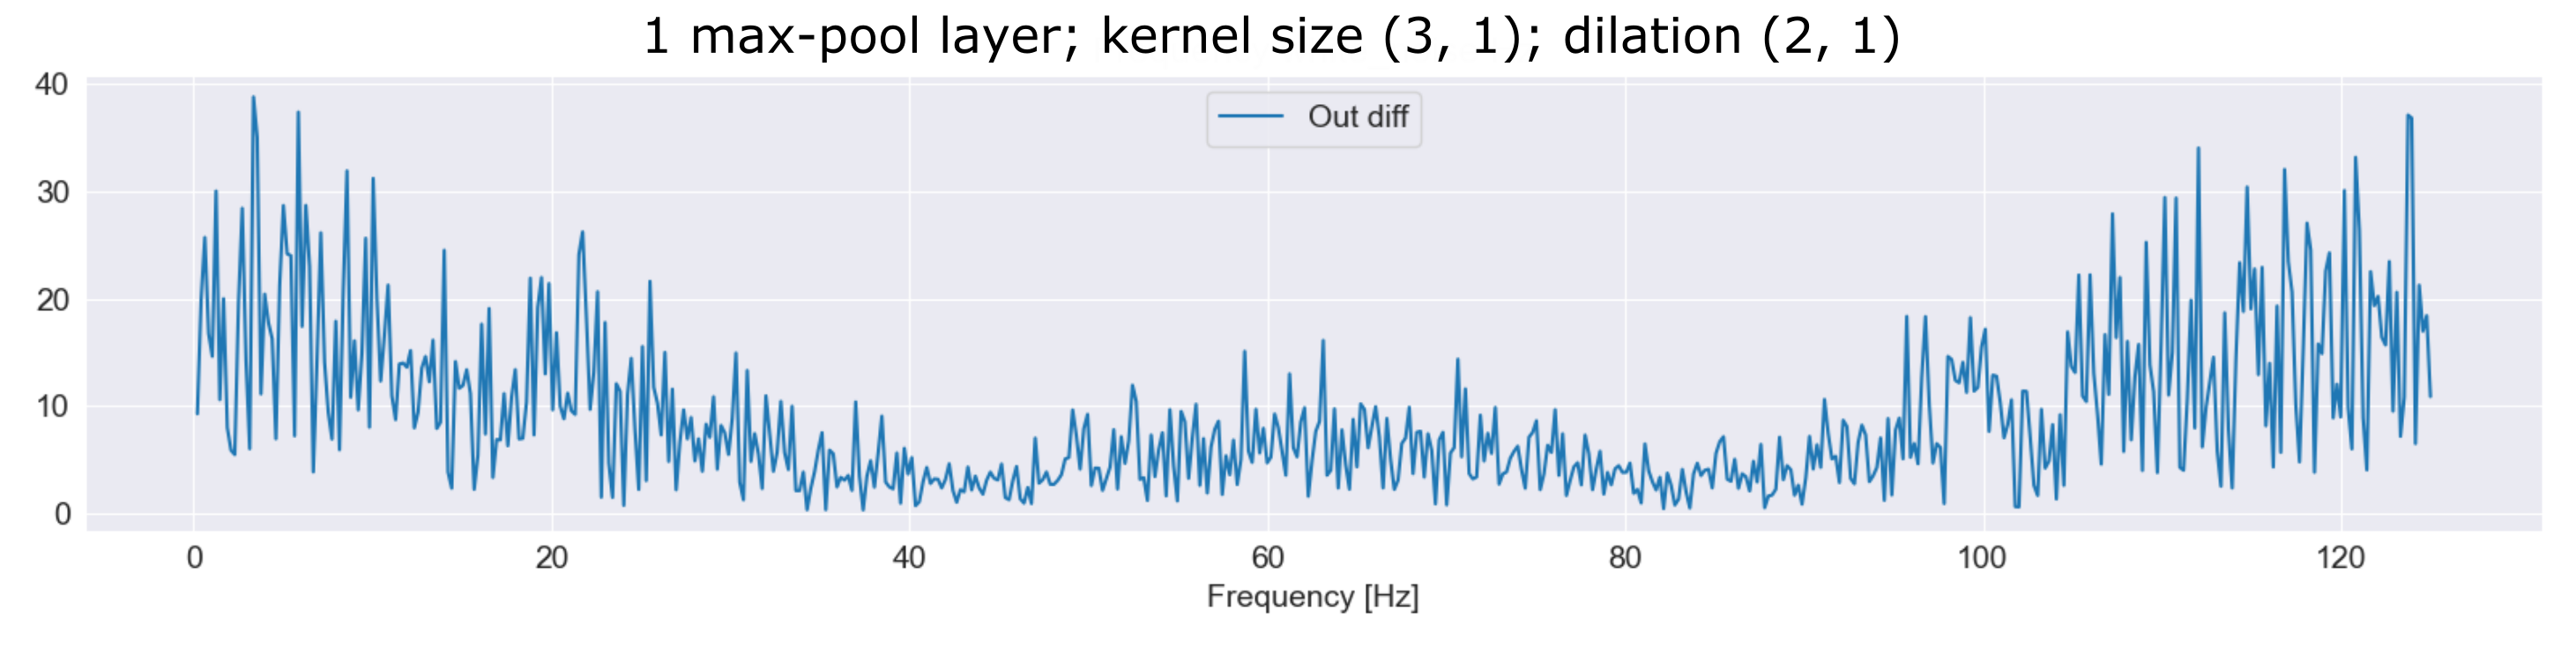
\includegraphics[width=1\linewidth]{img/ch4/absVel-maxpool-k3-d2}
   \caption{}
   \label{fig:Ng2}
\end{subfigure}

\caption[]{}
\end{figure}\label{fig:max-pool-changes}

The conclusions that can be made about the gradients peak when changing the kernel sizes and dilations of the max-pool layers are summarized below.
The majority of the above presented results suggests that the gradient peak is indeed the architecture artifact.
Its disappearance without loss of performance and the behaviour of the output signal when passed through single layers are in line with the hypothesis about frequency alignment.
The fact that the different kinds of channels (motor, non-motor) have similar gradient values at the peak also suggests that it only emerges because of the alignment.
If the motor channel gradients for the peak were visibly larger, it would support the hypothesis that some useful information is in this peak.
But because they are almost equal we can deduce that it is likely caused by the frequency alignment which should affect all channels in the same way.
The only argument speaking in favor of the gradient peak being informative for the network when making its decision is its amplification with training.
Nevertheless, this can be also attributed to the network not amplifying the peak but not actively working to suppress it as it occurs naturally when the signal passes through max-pool layers.
Lastly also the fact that the peak is also visible only when the input window is shortened to give only one output diminishes the credibility of the peak containing information useful for decoding.
Without the averaging, the gradient method is less stable and therefore also less reliable.
Overall, the gradient peak definitely cannot be taken as proof that the network is using high-gamma.

\section{Architectural modifications}\label{sec:architectural-modifications}
\subsection{Performance}\label{subsec:performance}
While the gradient peak seemed like a dead end, while studying it, we noticed that some of the networks, especially those with smaller kernel sizes and/or dilation parameters in their max-pool layers seem to perform significantly better.
Therefore, we decided to do a thorough inspection of how each of the networks performs on the filtered datasets as described in Section~\ref{subsec:modifications-to-the-dataset}.
The results can be seen in Figure~\ref{fig:original-performances-velocity} for velocity and Figure~\ref{fig:original-performances-absolute-velocity} for absolute velocity.
In the following points we summarize the findings on the different datasets.

\begin{itemize}
    \item \textbf{Full training and validation} Some of the networks significantly outperformed the Deep4Net sbp0 when both trained and validated on full data. The best performing network was the network where the max-pool layer had no influence, namely the one with max-pool layer kernel size 1.
    \item \textbf{Full training and low-pass validation} When the networks were trained on the full dataset and validated on the low-passed dataset (< 40Hz), the performance changed significantly for all the networks as is obvious from the Figure~\ref{fig:original-performances}.
    Nevertheless, in order to achieve a statistically significant decrease in performance, we had to use a Butterworth filter of order 15 instead of order 3 which was previously used inZ\cite{Hammer-2021}.The 3rd order filter caused no apparent change in performances.
    The Butterworth filter gradually attenuates the frequencies above the cut-off frequency (40Hz in this case).
    The higher the filter order, the steeper the attenuation is.
    Therefore, the fact that the performance decrease followed only after the stronger filter was employed suggests, that the network indeed focuses on frequencies above 40Hz but not particularly high frequencies (those in the high-gamma band) which were attenuated by both the 3rd as well as 15th order filter Figure~\ref{fig:filters}.
    \item \textbf{High-pass training and validation} To see if the networks are able to use information from the high-gamma frequency band at all, the networks were trained and evaluated on the high-pass dataset (>60Hz).
    As is clear from Figure~\ref{fig:original-performances}, the networks are able to use some information from the high-gamma especially when decoding absolute velocity where the correlations are often not only significantly above chance decoding but also achieve fairly good correlation coefficients.
    \item \textbf{Full training and high-pass validation} A possibility to find out if the networks when trained on full data are learning from the high-gamma frequency band, is to train the network on the full dataset and validate only on the high-passed data.
    Therefore we also explored this option.
    It is obvious from Figure~\ref{fig:original-performances} that only few networks perform significantly better than chance level decoding.
    The conclusion that the network, when given access to, utilizes primarily information from the low end of the frequency spectrum can be drawn from this result.
    \item \textbf{Low-pass training and high-pass validation}
    Training on low-passed data and validation on high-passed data was also important to further study how the network operates.
    We wanted to find out if it is able to somehow transfer information between two completely separate datasets.
    Because the cut-off frequency for the low-passed data is 40Hz and for the high-passed data 60Hz with a very steep filter, there is no frequency overlap between the two sets.
    Therefore, it would be interesting but also rather surprising if from modulation in the low frequencies (below 40Hz) the network would learn to use information about modulations in the high frequencies (above 60Hz).
    Nevertheless, as obvious from Figure~\ref{fig:original-performances}, the networks were unable to transfer any information.
    
\begin{figure}[!htpb]
\centering
\begin{subfigure}[b]{\textwidth}
   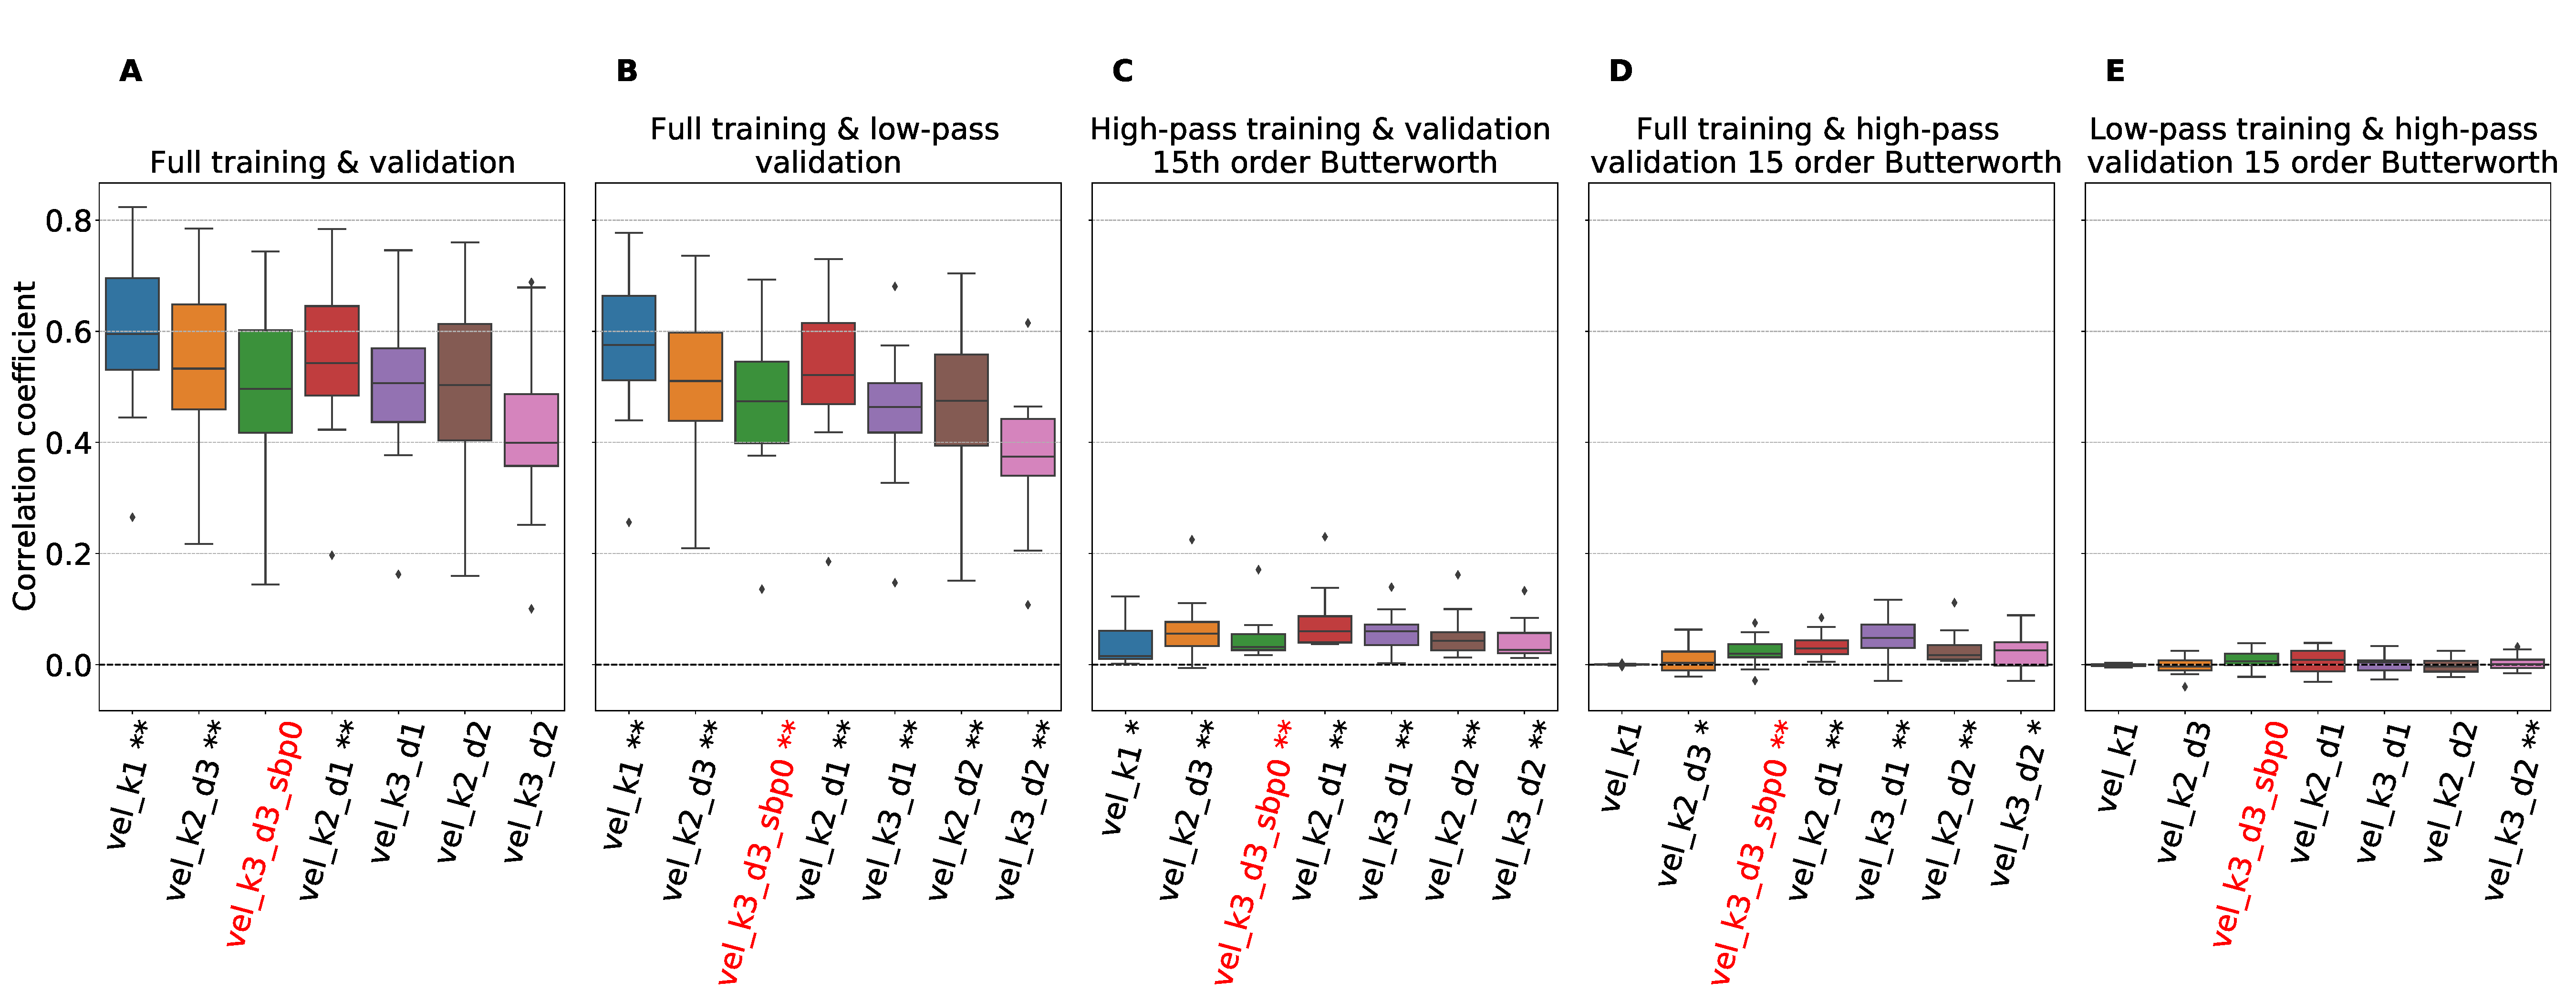
\includegraphics[width=1\linewidth]{img/ch4/original_setting_vel_performance_comparison}
   \caption{}
   \label{fig:original-performances-velocity} 
\end{subfigure}

\begin{subfigure}[b]{\textwidth}
   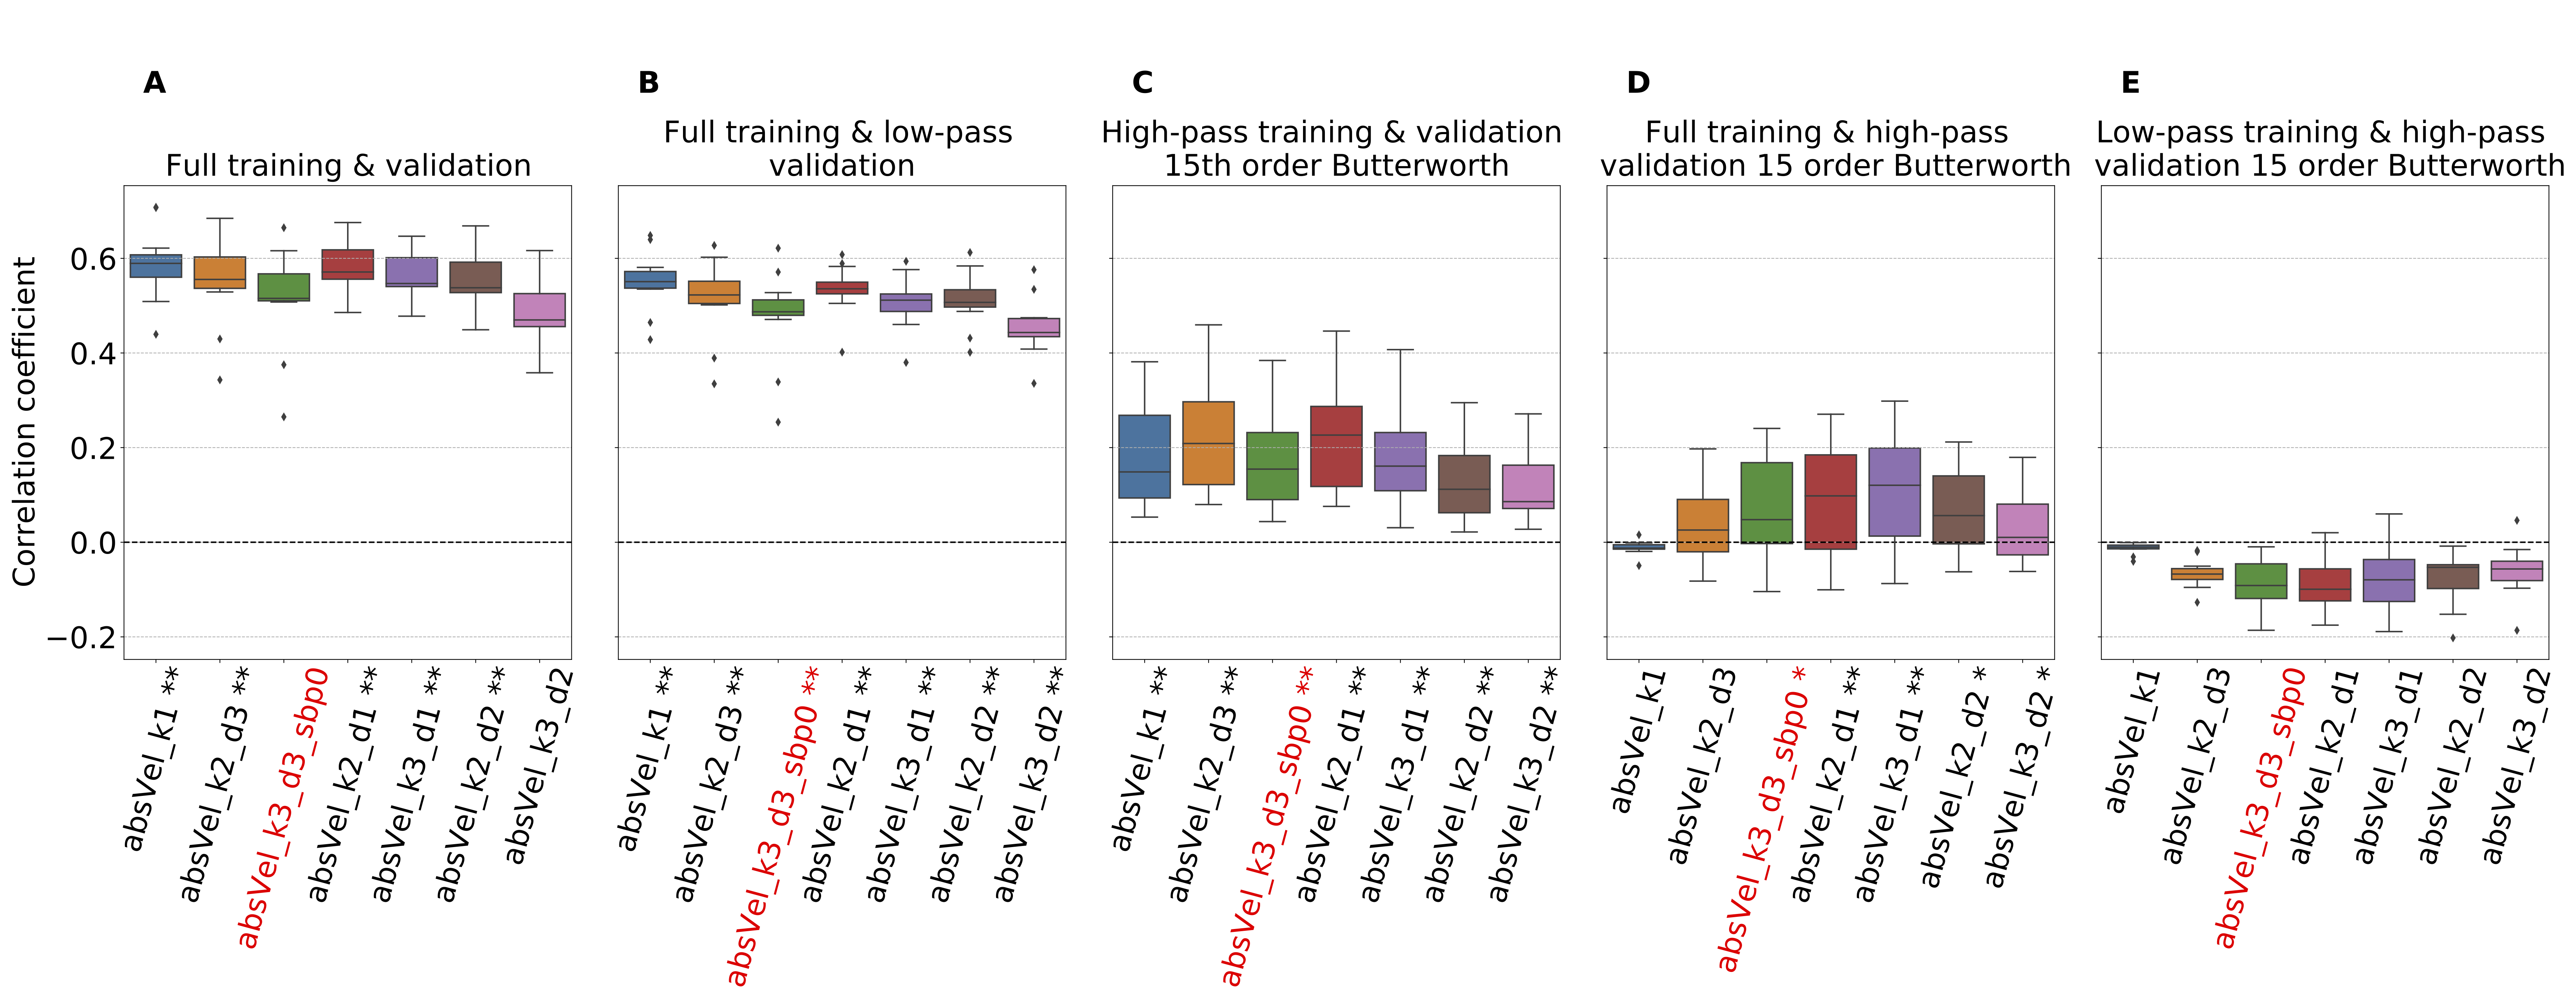
\includegraphics[width=1\linewidth]{img/ch4/original_setting_absVel_performance_comparison}
   \caption{}
   \label{fig:original-performances-absolute-velocity}
\end{subfigure}
\caption[]{}
\end{figure}\label{fig:original-performances}


\end{itemize}

The findings presented in this section lead to two interesting questions.
The first one  is what do the gradients of the various architectures look like and do some of them use high-gamma?
This analysis is described in Section~\ref{subsec:gradients}.
The second question that arises if we notice, that the performance seems to drop with increasing size of the receptive field \cref{fig:distance-from-rf}.
Networks with a smaller receptive field seem to perform better possibly because the predicted time-point is closer to the centre of the receptive field.
Therefore, it is interesting to see what happens when we shift the predicted time-point to the centre of the receptive field.
More details and the analysis are described in Section~\ref{sec:shifting-the-predicted-time-point}.

\begin{figure}[!htpb]
\centering
\begin{subfigure}[b]{0.65\textwidth}
   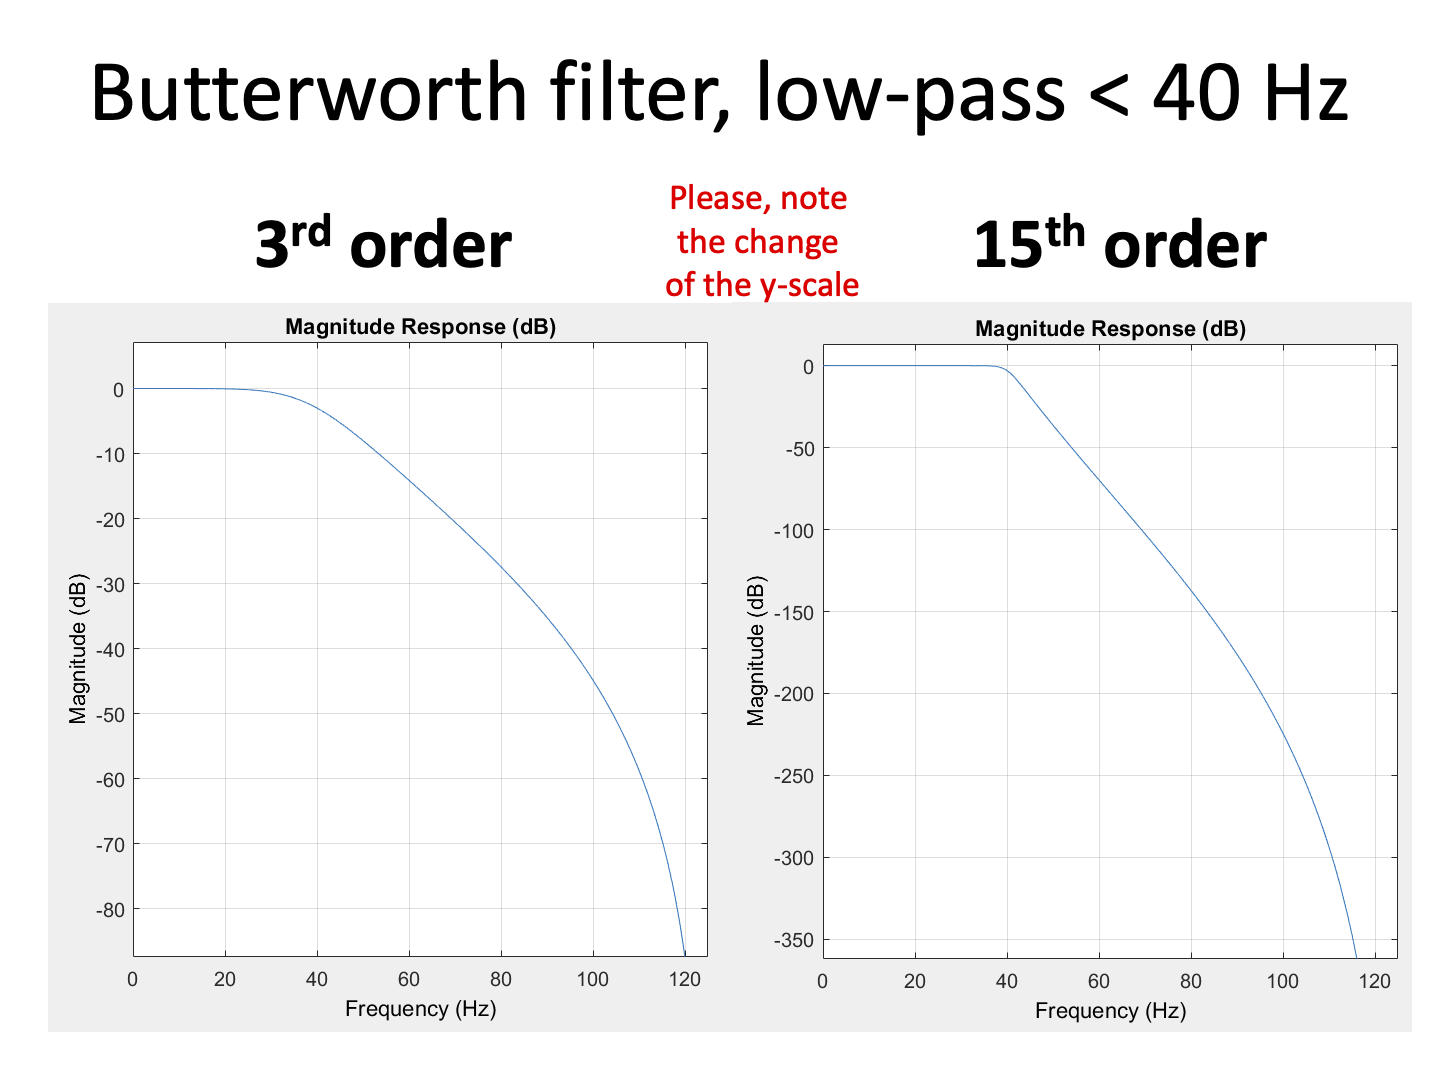
\includegraphics[width=1\linewidth]{img/ch3/lp-butterworth-filter}
   \caption{}\label{fig:lp-filters}
\end{subfigure}

\begin{subfigure}[b]{0.65\textwidth}
   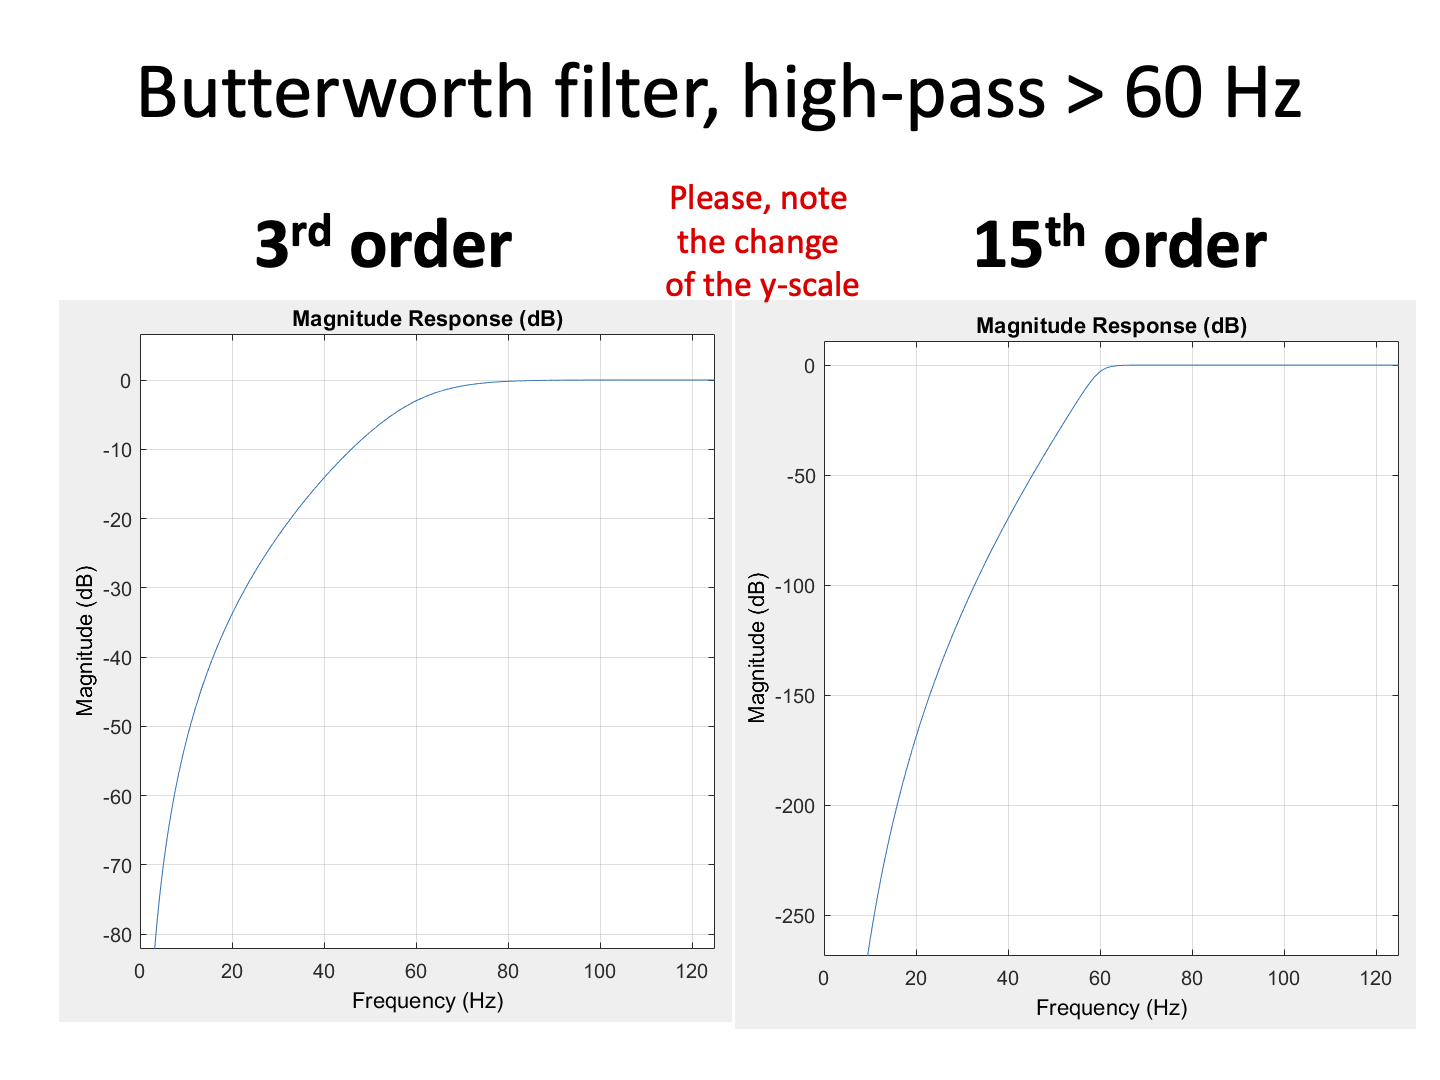
\includegraphics[width=1\linewidth]{img/ch3/hp-butterworth-filter}
   \caption{}
\end{subfigure}
\caption[]{}\label{fig:hp-filters}
\end{figure}\label{fig:filters}

\subsection{Gradients}\label{subsec:gradients}
The differences in performance among the networks, reinforce the interest in the gradients of the various architectures.
Since some of the networks perform significantly better compared to the initial Deep4Net, we analyze gradients of the different architectures to see if the reason for a better performance is their ability to use information from the high-gamma band.
We perform the gradient visualization of all the architectures with kernel sizes 1, 2 and 3 and dilations as powers of 1, 2 and 3.

The results show differences in gradients among the architectures.
Gradients of all intermediate layers and the visualizations can be found in the Appendix.
Figure~\ref{fig:last-layer-grads} includes the gradients of the output layer which in our opinion best represents the gradients of the other layers for all the architectures.

\begin{figure}[!htpb]
\centering
\begin{subfigure}[b]{\textwidth}
   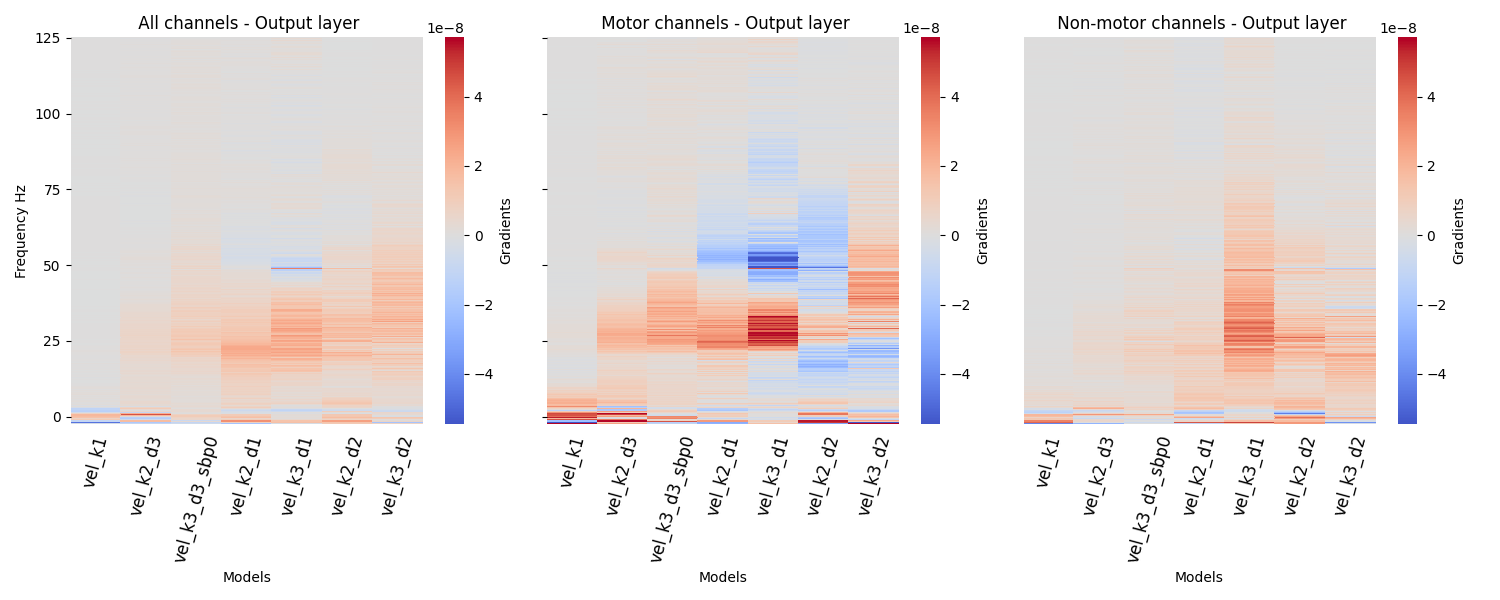
\includegraphics[width=1\linewidth]{img/ch4/vel-last-layer-grads}
   \caption{}
\end{subfigure}\label{fig:absVel-last-layer-grads}

\begin{subfigure}[b]{\textwidth}
   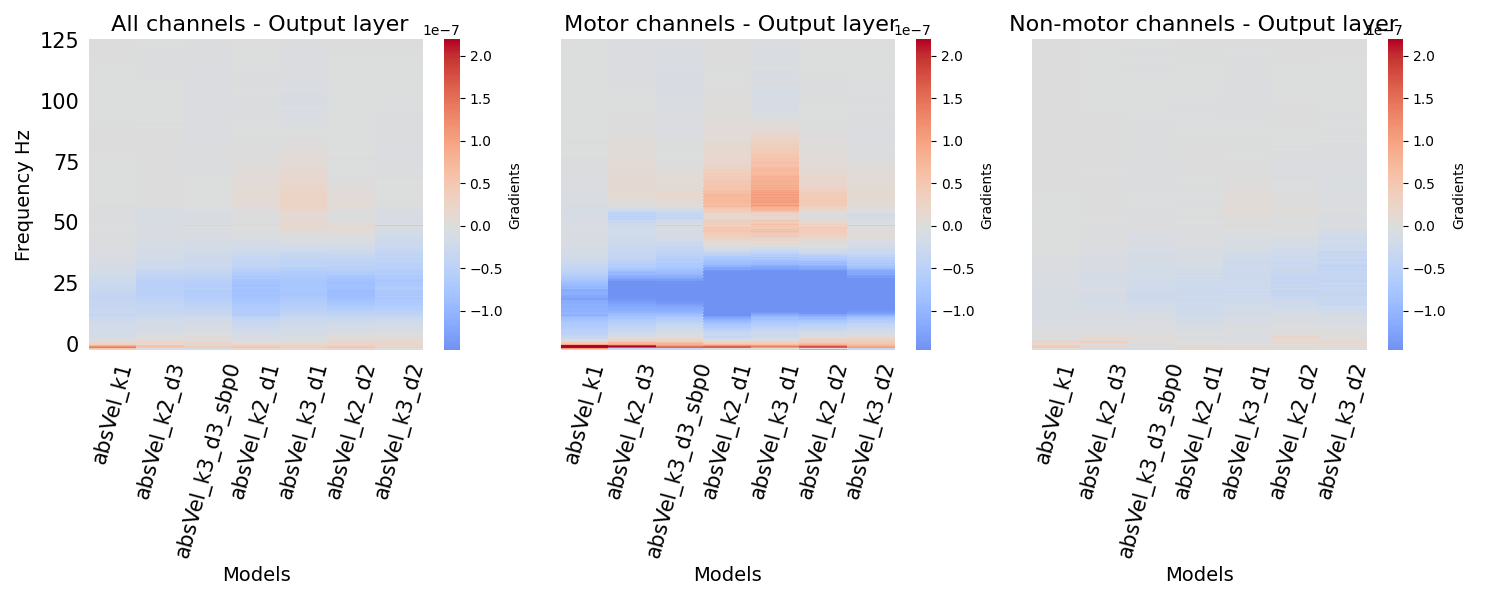
\includegraphics[width=1\linewidth]{img/ch4/absVel-last-layer-grads}
   \caption{}
\end{subfigure}\label{fig:vel-last-layer-grads}
\caption[]{}
\end{figure}\label{fig:last-layer-grads}

Based on the performances of the networks presented in Section~\ref{subsec:performance} and the gradients presented in this Section these important and interesting observations can be made:

\begin{itemize}
    \item The networks focus on motor-channels when making predictions.
This is to be expected when they are tasked with decoding movement.
    \item There are obvious differences between the gradients for velocity and absolute velocity.
    Nevertheless, for both variables the network without max-pool, here denoted as {variable}\_k1 is the best performing architecture.
    And it is in both cases also the network which is most interested in modulations in the low frequency bands.
    This suggests that using the information in the high-gamma frequency band is not necessarily an asset.
    \item The networks which exhibit higher interest in information from the higher frequencies, namely the k2\_d1, k3\_d1 and k2\_d2 are also those, which are able to perform significantly above chance when trained on full data and validated on high-passed data.
    This suggests consistency between the gradient visualization and the performance analysis.

\end{itemize}


\section{Shifting the predicted time-point}\label{sec:shifting-the-predicted-time-point}
In this section we describe how the performance and gradients change when the predicted time-point is shifted with respect to the receptive field.
Two kinds of analyses are introduced here.

\begin{enumerate}
    \item Shifting the predicted time-point to the centre of the receptive field
This analysis was performed on all the network architectures and compares how the different architectures react to the shift both performance-wise and gradient-wise.
We highlight the differences and similarities between the architectures.
    \item Shifting the predicted time-point in steps across the receptive field
This analysis was performed only on the original Deep4Net sbp0.
It compares how the performance and gradients of the network change when the predicted time-point is shifted across the receptive field using a different ratio of information from the future and from the past.
\end{enumerate}


\subsection{Shifting the predicted time-point to the centre of the receptive field}\label{subsec:shifting-the-predicted-time-point-to-the-centre-of-the-receptive-field}
An important observation when looking at the performance of the different architectures described in Section\ref{sec:architectural-modifications} was made.
We noticed that the smaller receptive field seemingly correlates with a higher prediction accuracy especially for absolute velocity decoding.
To visualize this, we created Figure~\ref{fig:figure-distance} which sorts the different architectures based on the size of the receptive field from smallest to largest and plots the average correlation coefficient each of these networks achieved.
There is a clear descending pattern especially for absolute velocity where the only exceptional network is the k2\_d3 network which performs well with a large receptive field.

\begin{figure}
\centering
   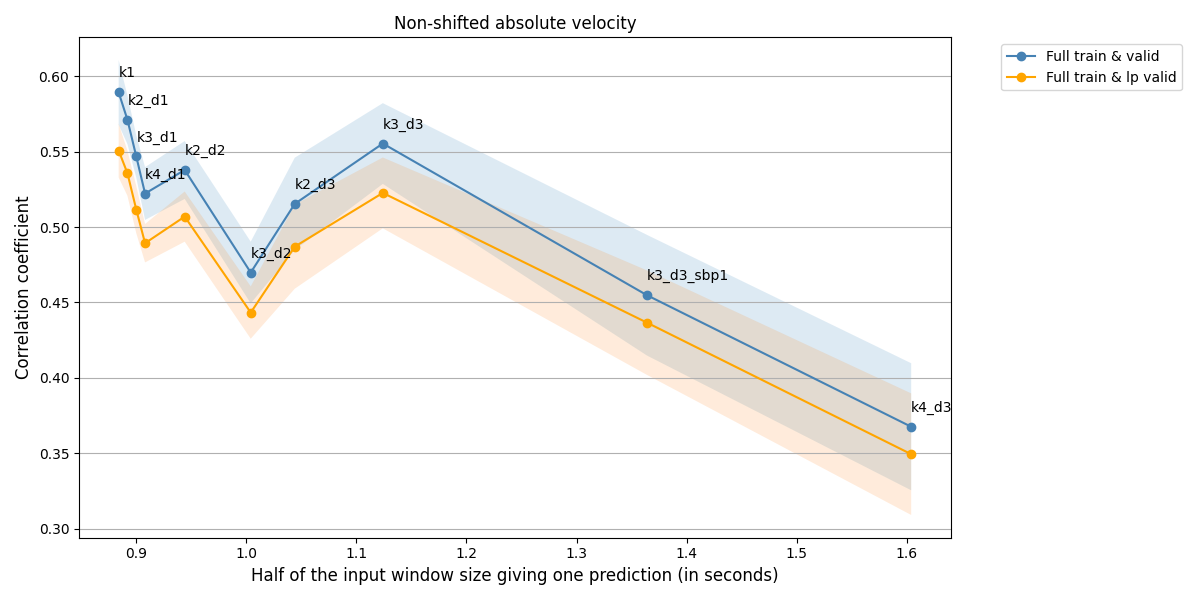
\includegraphics[width=1\linewidth]{img/ch4/distance-shifted-performance-absVel}
   \caption{}
\end{figure}\label{fig:figure-distance}

This finding further corroborates the idea to shift the predicted time point to the center of the receptive field.
The receptive field as described in Section~\ref{subsec:receptive-field} is non-uniform.
It considers mostly input-points in its centre while in the original decoding, the predicted time-point is located just outside the receptive field.
Therefore, we shift the inputs and prediction so that the iEEG signal, which was recorded at the same time as the predicted movement was executed, is in the centre of the receptive field and present how this affects the performance and gradients of the various architectures.
This causes the procedure to be unsuitable for online BCI because half of the input window uses information from the future.
\subsubsection{Performance}
The results can be seen in Figure~\ref{fig:shifted-performance}.
It is obvious that the shift greatly improves performance of all the networks and the performance differences between the architectures are diminished.
Notably the performance of the networks on the high-gamma dataset also increased especially for absolute velocity.
\begin{figure}[!htpb]
\centering
\begin{subfigure}[b]{\textwidth}
   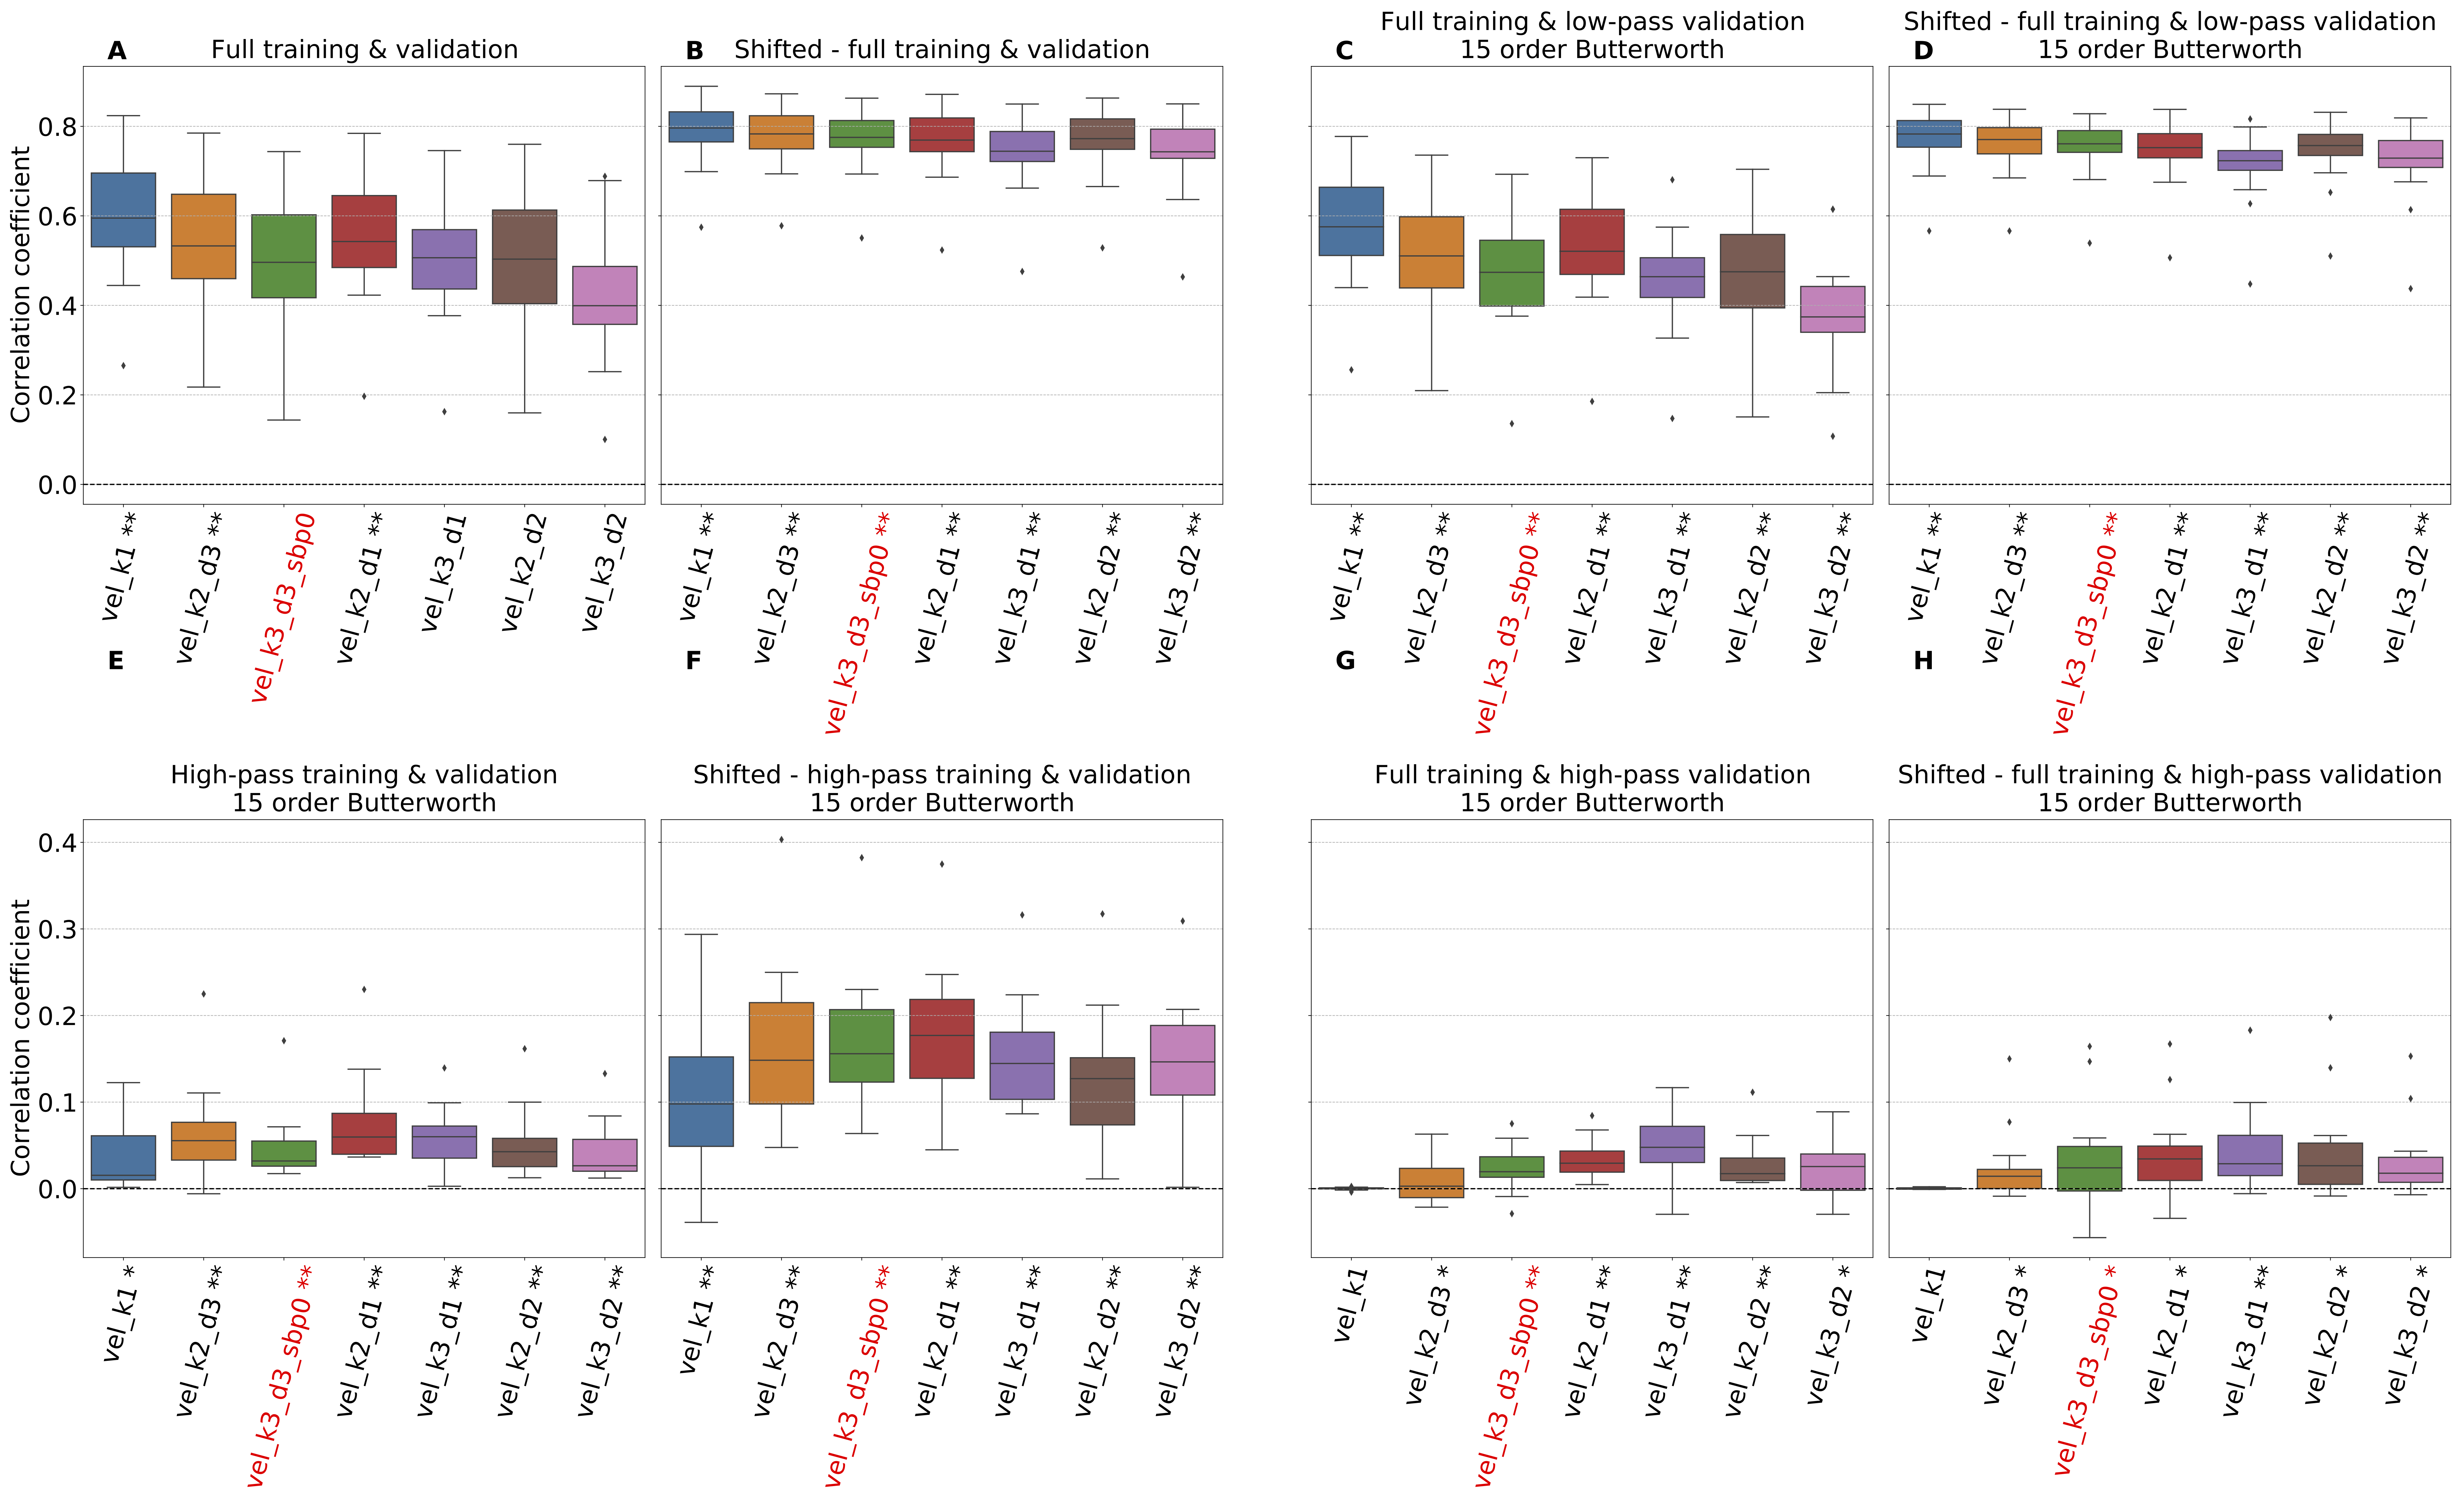
\includegraphics[width=1\linewidth]{img/ch4/shifted_vs_non_shifted_vel_performance_comparison}
   \caption{}
\end{subfigure}\label{fig:shifted-performance-vel}

\begin{subfigure}[b]{\textwidth}
   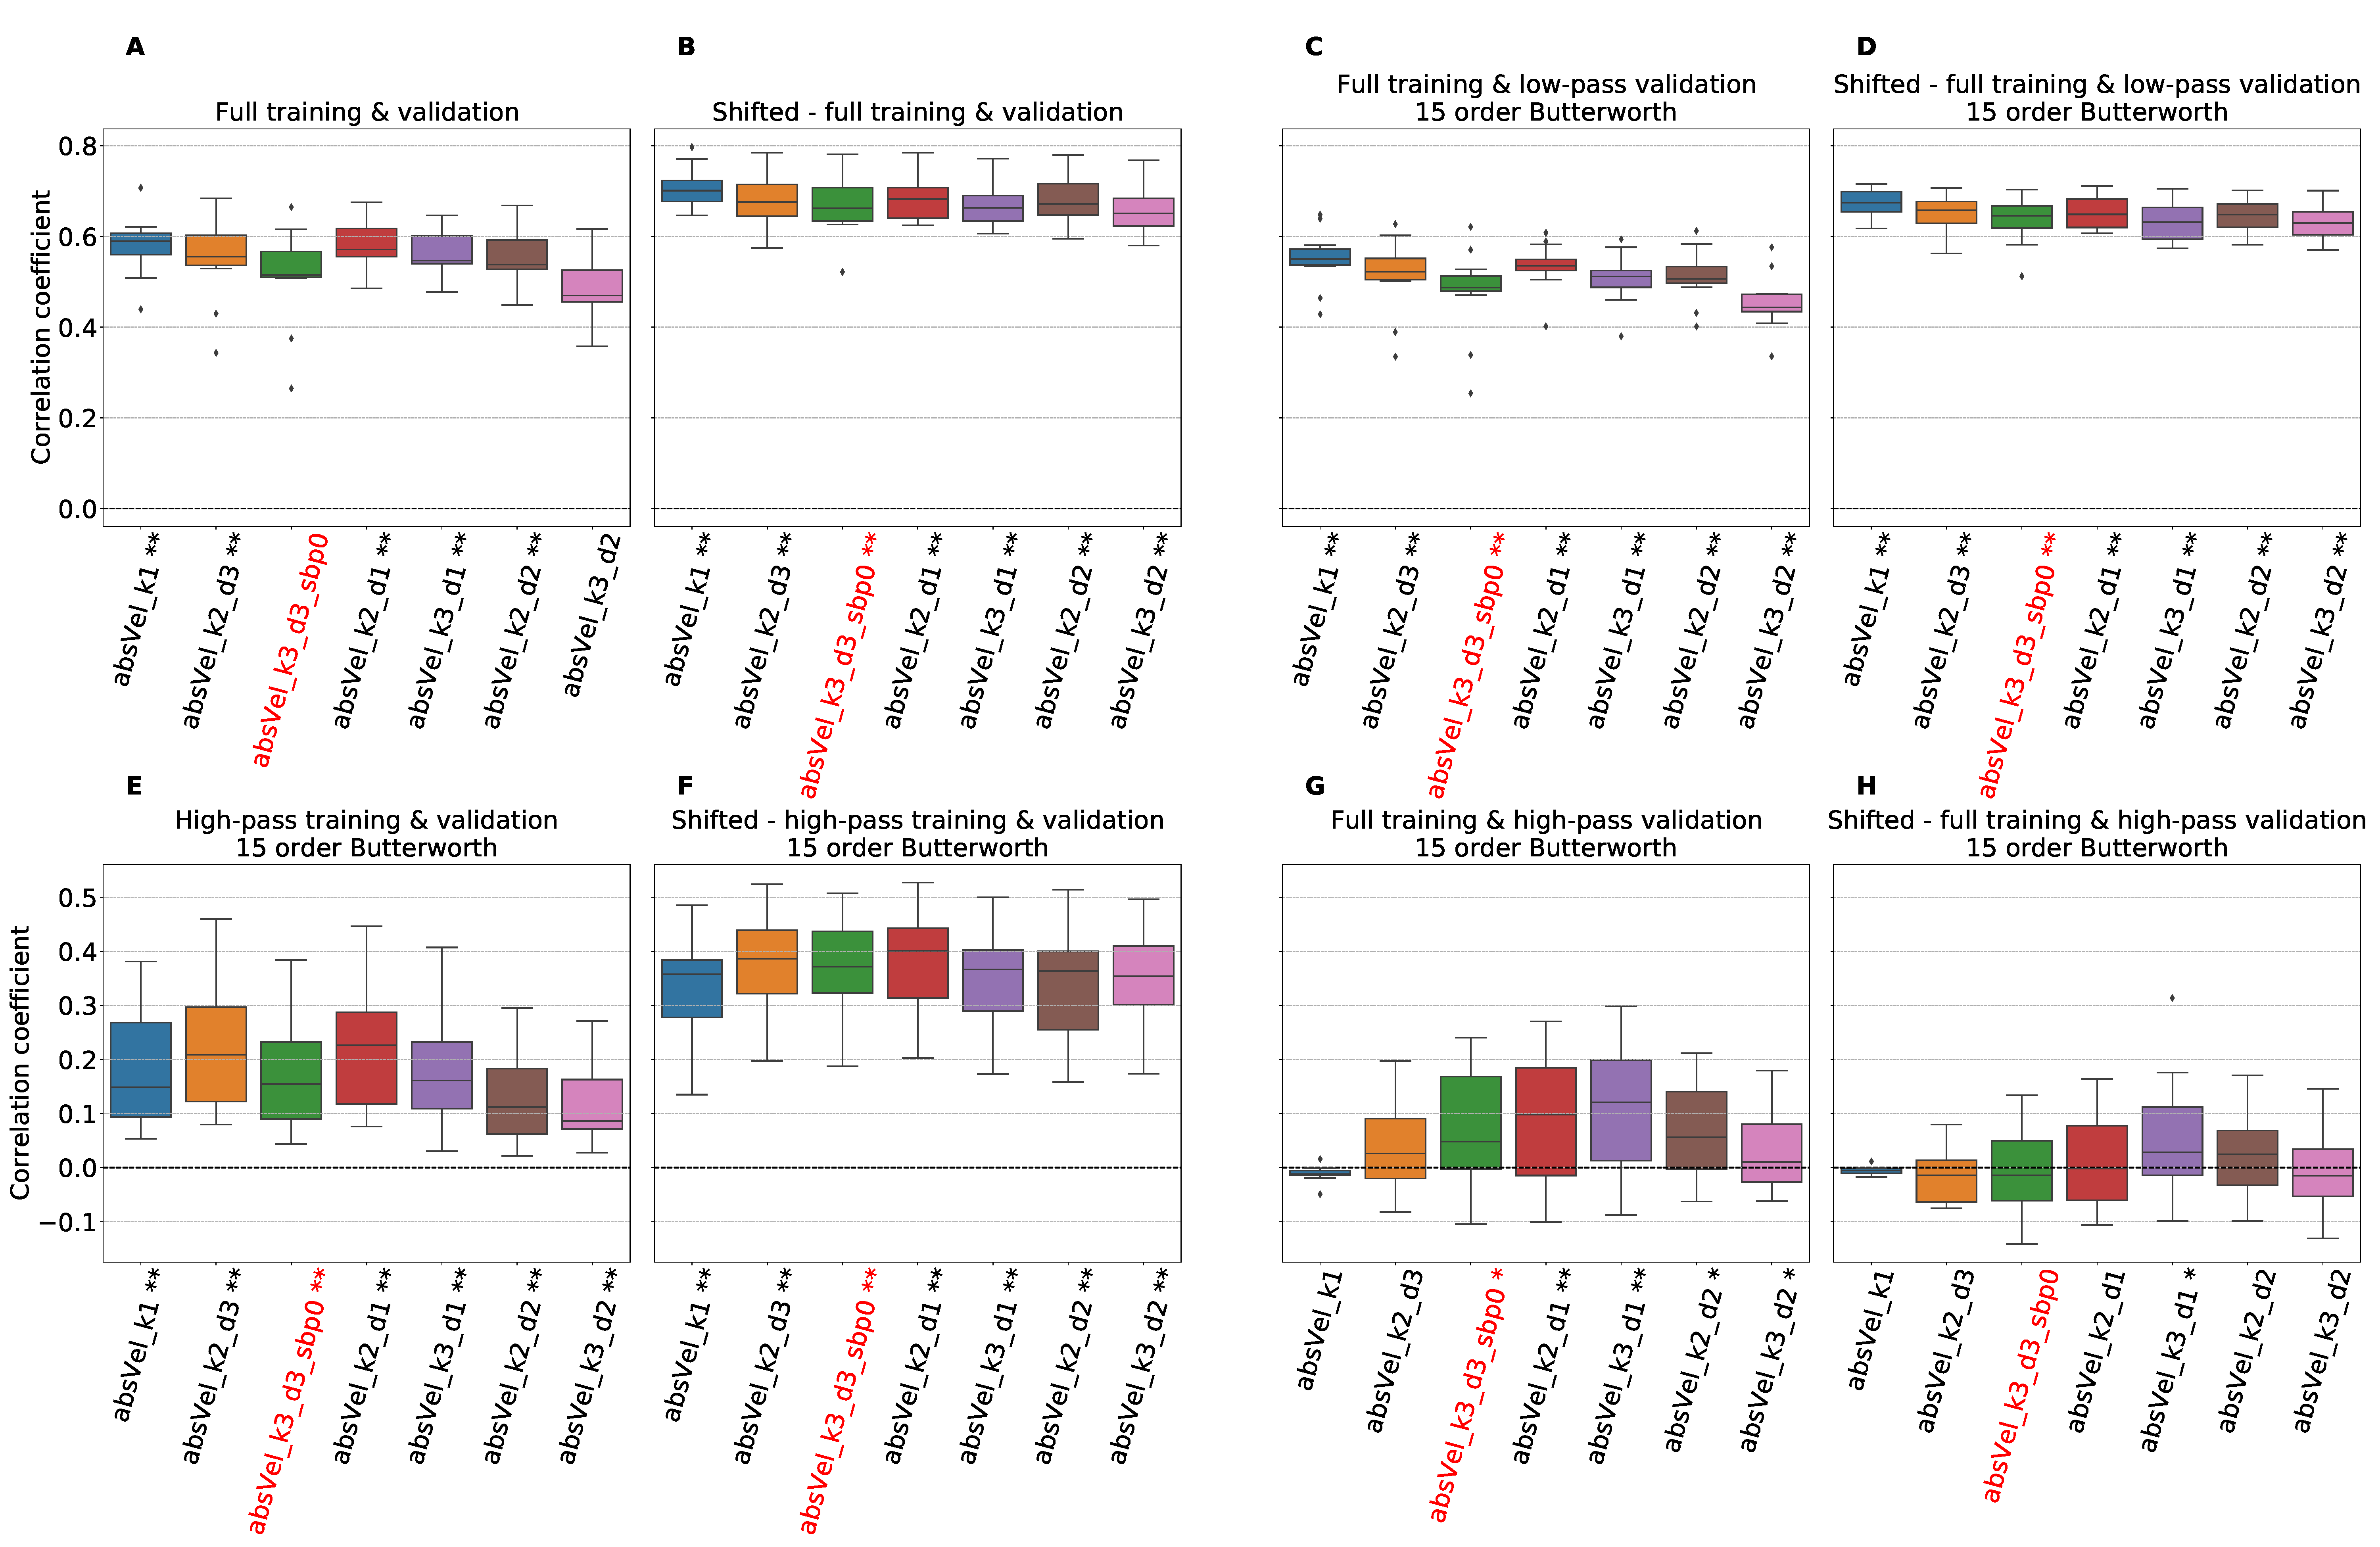
\includegraphics[width=1\linewidth]{img/ch4/shifted_vs_non_shifted_absVel_performance_comparison}
   \caption{}
\end{subfigure}\label{fig:shifted-performance-absVel}
\caption[]{}
\end{figure}\label{fig:shifted-performance}

The improvement can be caused by two things:
\begin{enumerate}
    \item By the network being able to focus on signals recorded directly before the movement execution.
    \item By the network having access to information from the future.
\end{enumerate}

We hypothesise that is most likely a combination of the two.
Conclusion about how much each of the above described influences the prediction improvement cannot be made from the presented experiments.
It would be interesting to build a network with a uniform receptive field and then conduct experiments which would clarify this.
Nevertheless, such an analysis is out of the scope of this thesis.

\subsubsection{Gradients}
In Section~\ref{subsec:gradinet-visualization} we already saw that the best performing networks are those which use lower frequencies.
Here we show, how the shift influences the gradients.
Hypothetically, the information about the movement in high-gamma could be informative only in the moments directly preceding the movement.
Therefore the networks are unable to use it because they focus on the signal recorded too far in the past.
To test this hypothesis, we visualize the gradients of the networks trained in the shifted settings.

We compare the gradients between the networks in the original non-shifted setting and the shifted setting where the predicted time point is in the centre of the receptive field.
This was analysis was performed for all the architectures for all their intermediate layers on 1. the full dataset and 2. the high-passed dataset.
The complete results can be found in the Appendix.
Here, we show results from the third convolutional layer which servers as good representation of the overall trend~\ref{fig:}
The trends are different for the full dataset and the high-passed dataset.

\begin{enumerate}
    \item Gradients of networks which are \textbf{trained and validated on full data} are displayed in Figures~\ref{fig:vel-shifted-vs-non-shifted-grads} and \ref{fig:absVel-shifted-vs-non-shifted-grads}.
    What we observe is that the networks across all architecture seem to refine their focus to more narrow frequency bands.
    For example the vel\_k1 network which is the one without max-pools has high-gradient values in the original setting for frequencies up to 25Hz when looking at gradients for motor channels.
    In the shifted setting the band with high gradient values narrows to frequencies closer to 0.
    The network vek\_k2\_d2 is in the non-shifted setting focused mostly on frequencies between 25 and 60 Hz. Nevertheless, with shifting the gradients for a lot of frequencies the width of the band is reduced, and the network focuses on frequencies around 25Hz. For no network did the shift cause an increase in the use of information from the high-gamma frequency band.
    Rather it seems, that the shift allowed access to less noisy information in the clearly informative bands such as the alpha and beta bands, and the network did not have to compensate with information from other frequencies.
    \item Networks which were \textbf{trained and validated on high-passed data} can be found in Figure \ref{}.
    Again, we only chose to display gradients of one layer to illustrate a behaviour shared by all layers. The gradients of the remaining layers can be found in Appendix \ref{}.
    What we observe in the gradients of the networks trained on high-passed datasets is different from what we observe on gradients of networks trained on full datasets, maybe even the opposite.
    The networks trained on shifted data exhibit interest in the same or a broader range of frequencies above the 60Hz cut-off frequency than the networks trained in the original, non-shifted setting.
    This and the increase in performance on high-passed datasets suggests that indeed the information from the future or directly preceding the movement contains more information about movement in the high-gamma band.
    But the fact that the networks trained on full data do not use high-gamma, and their performance increases significantly compared to the non-shifted setting points to the information in high-gamma being informative but redundant when having access to information from all frequencies.
\end{enumerate}

\begin{figure}[!htpb]
\centering
\RawFloats
\begin{subfigure}[b]{\textwidth}
   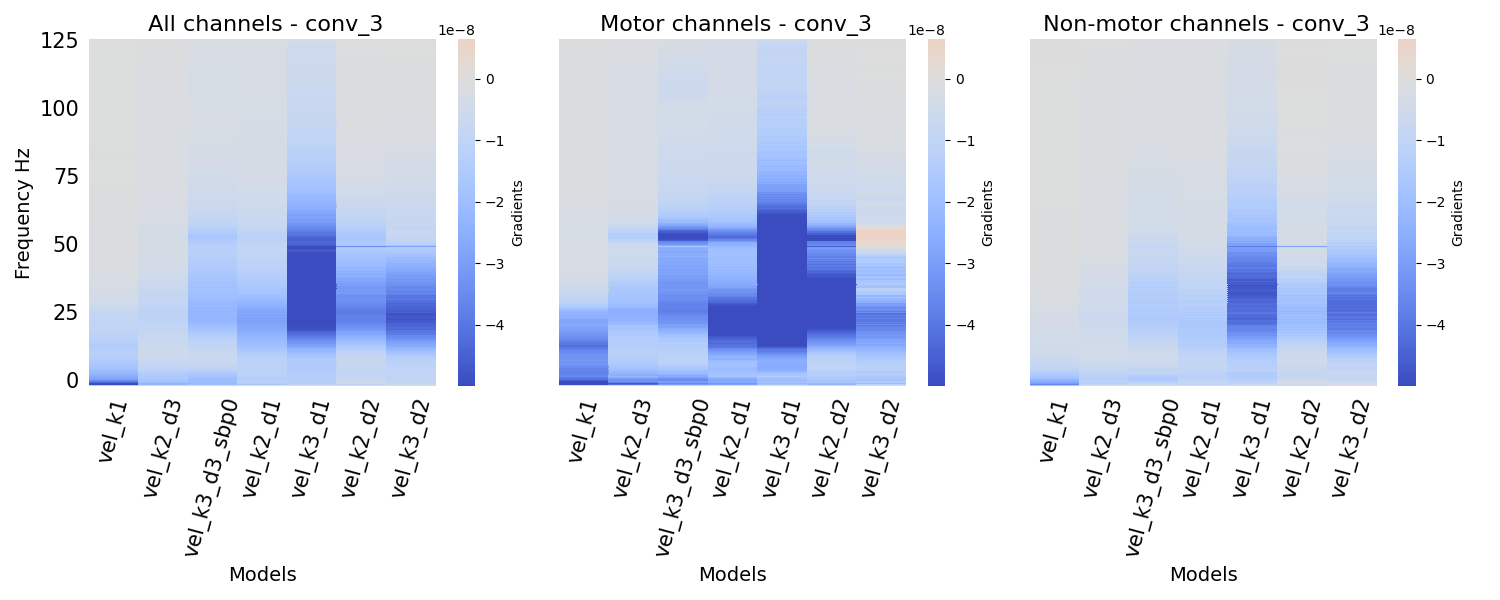
\includegraphics[width=1\linewidth]{img/ch4/vel-conv-3-layer-grads}
   \caption{}
\end{subfigure}\label{fig:vel-conv3-layer-grads}

\begin{subfigure}[b]{\textwidth}
   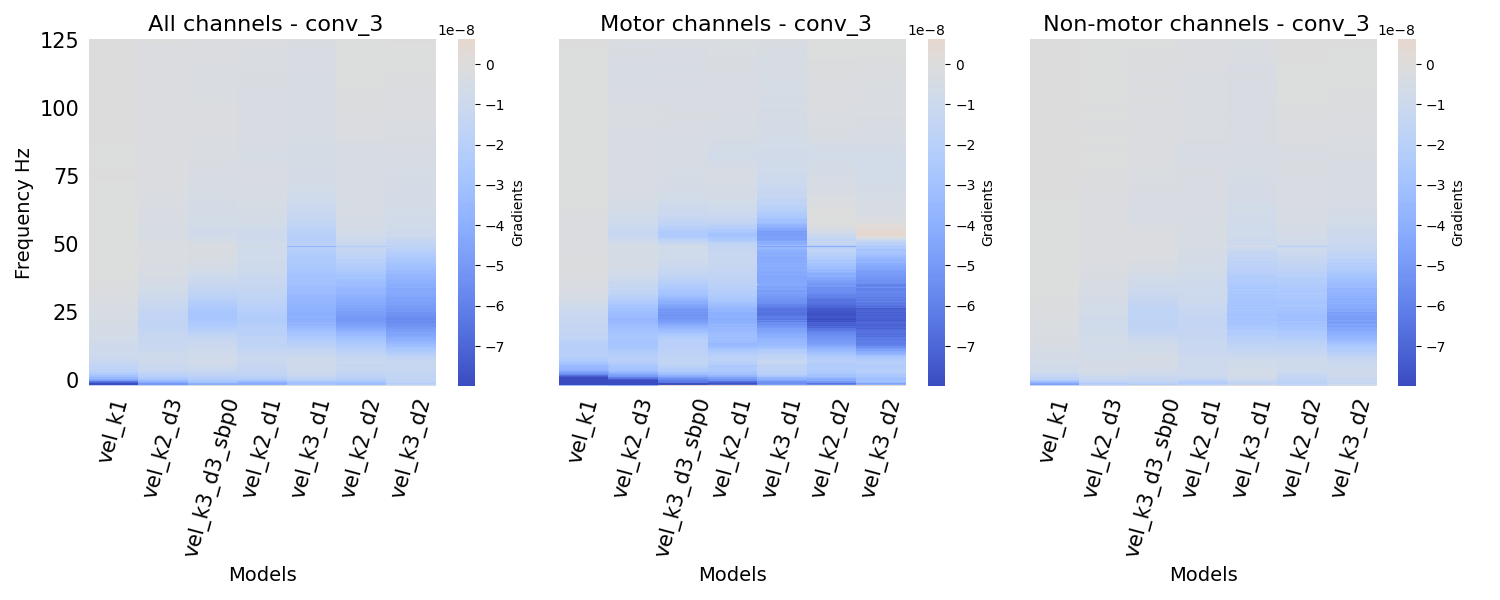
\includegraphics[width=1\linewidth]{img/ch4/vel-conv-3-layer-grads-shifted}
   \caption{}
\end{subfigure}\label{fig:vel-conv3-layer-grads-shifted}
\caption[]{}
\end{figure}\label{fig:vel-shifted-vs-non-shifted-grads}

\begin{figure}[!hpbp]
\begin{subfigure}[a]{\textwidth}
   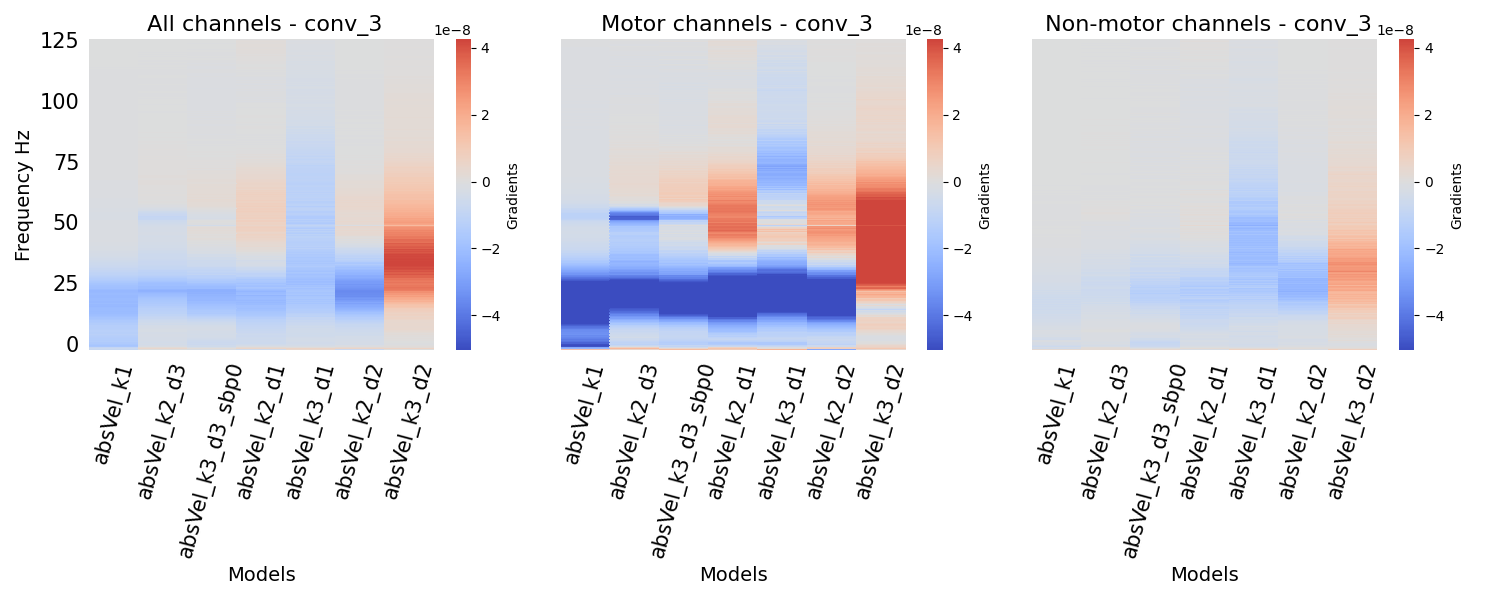
\includegraphics[width=1\linewidth]{img/ch4/absVel-conv-3-layer-grads}
   \caption{}
\end{subfigure}\label{fig:absVel-conv-3-layer-grads}

\begin{subfigure}[b]{\textwidth}
   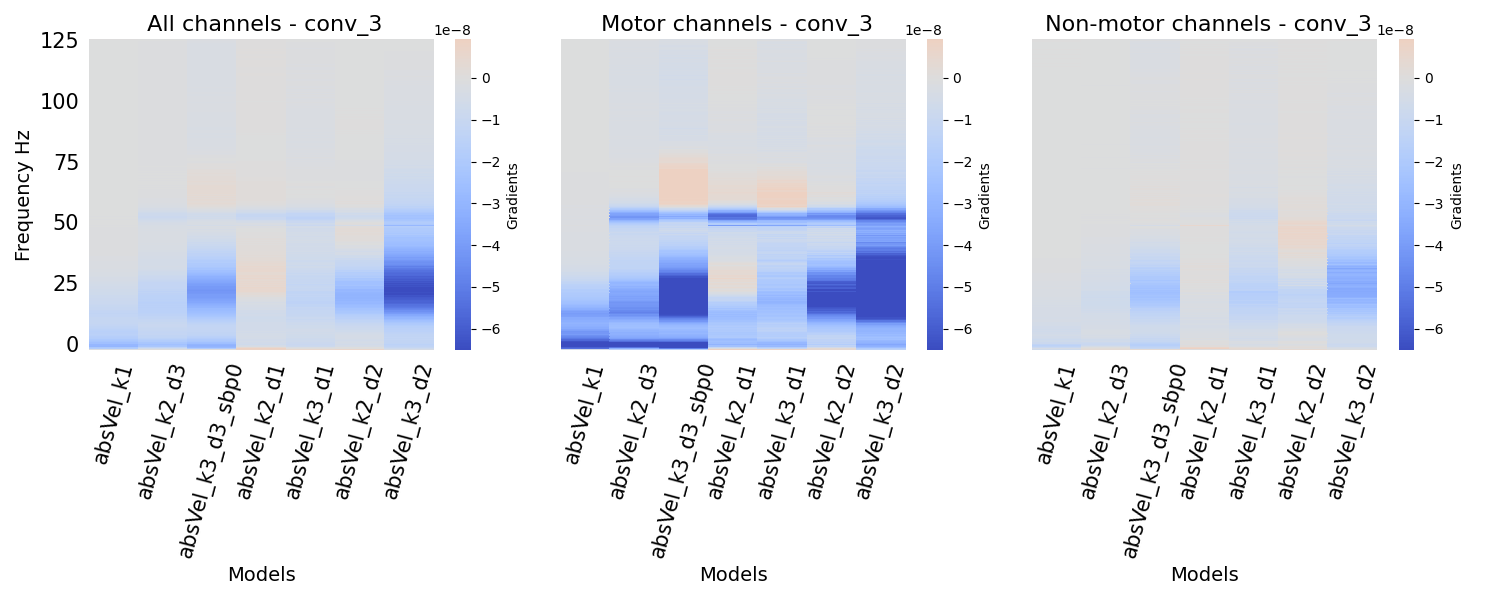
\includegraphics[width=1\linewidth]{img/ch4/absVel-conv-3-layer-grads-shifted}
   \caption{}
\end{subfigure}\label{fig:absVel-conv-3-layer-grads-shifted}
\caption[]{}
\end{figure}\label{fig:absVel-shifted-vs-non-shifted-grads}

% high-pass gradients with shift
\begin{figure}[!htpb]
\centering
\RawFloats
\begin{subfigure}[b]{\textwidth}
   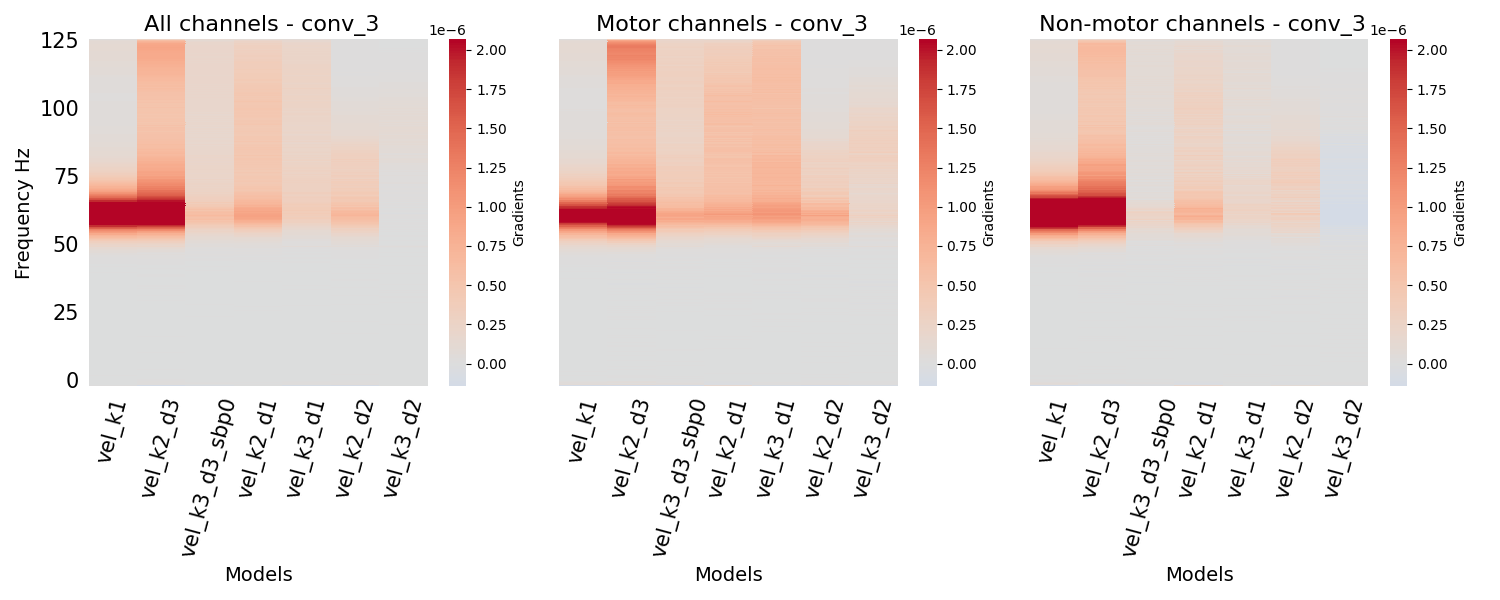
\includegraphics[width=1\linewidth]{img/ch4/vel-conv-3-layer-grads-hp}
   \caption{}
\end{subfigure}\label{fig:vel-conv3-layer-grads-hp}

\begin{subfigure}[b]{\textwidth}
   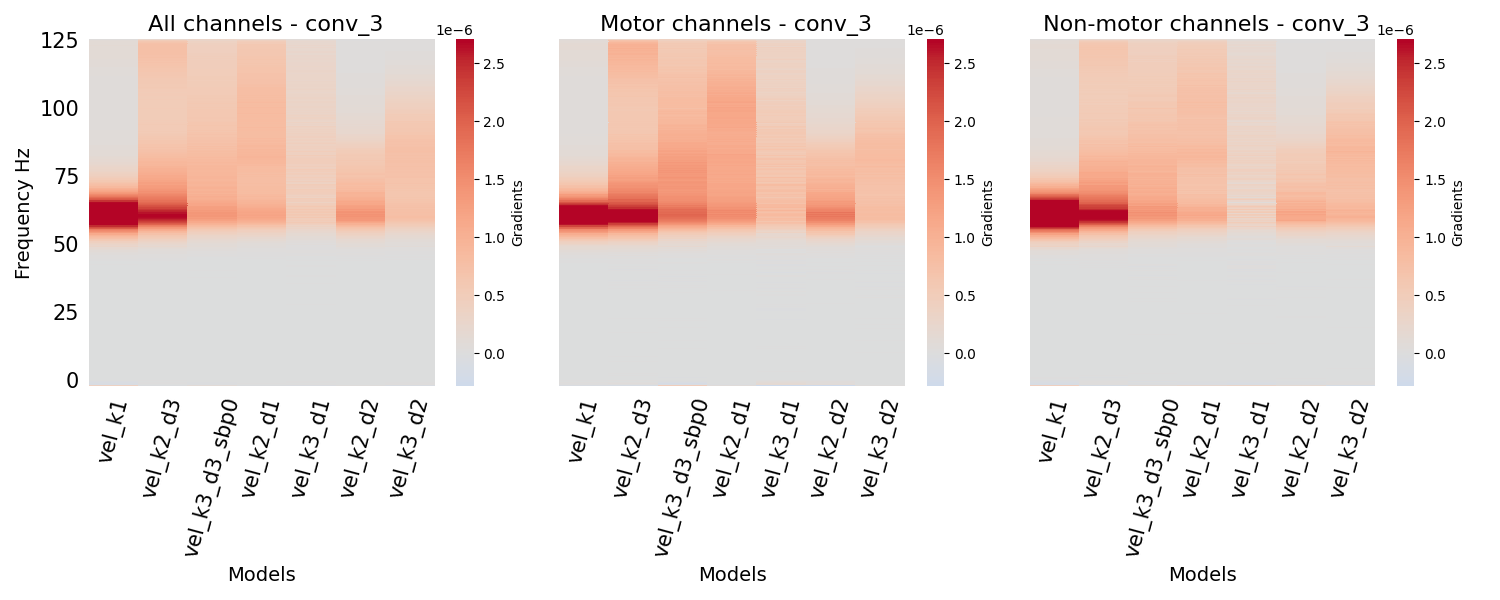
\includegraphics[width=1\linewidth]{img/ch4/vel-conv-3-layer-grads-hp-shifted}
   \caption{}
\end{subfigure}\label{fig:vel-conv3-layer-grads-shifted-hp}
\caption[]{}
\end{figure}\label{fig:vel-shifted-vs-non-shifted-grads-hp}

\begin{figure}[!hpbp]
\begin{subfigure}[a]{\textwidth}
   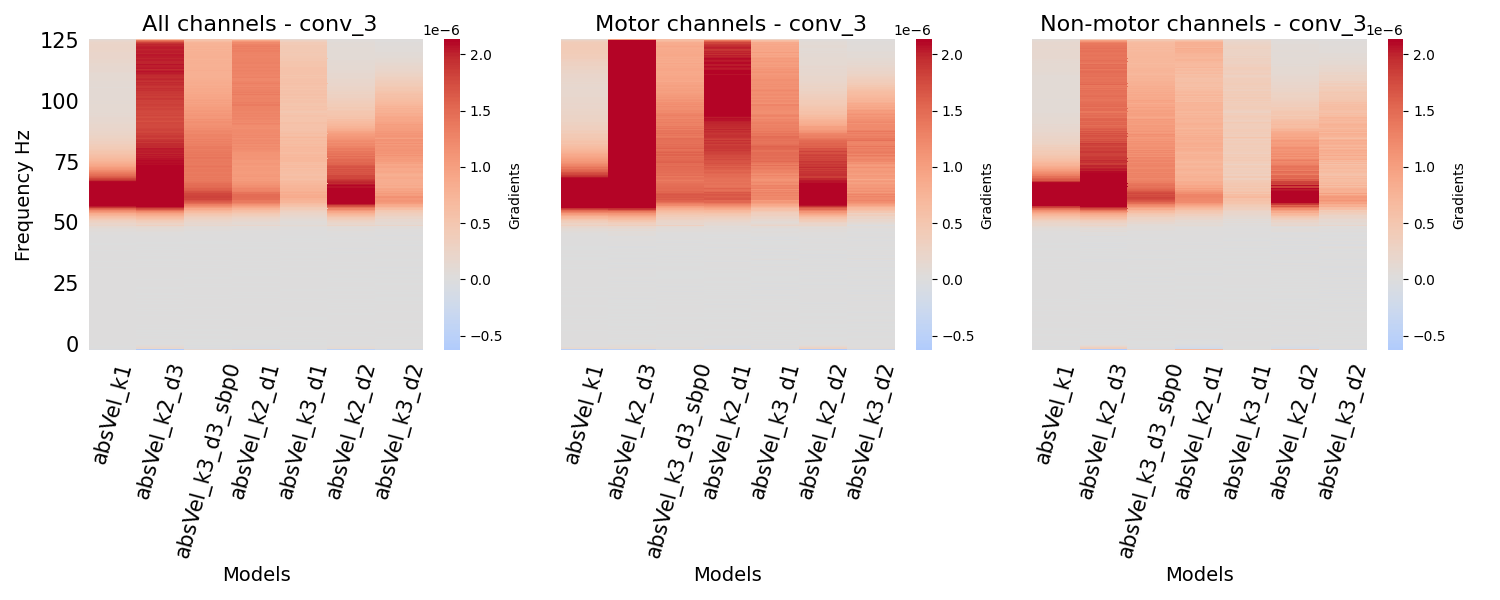
\includegraphics[width=1\linewidth]{img/ch4/absVel-conv-3-layer-grads-hp}
   \caption{}
\end{subfigure}\label{fig:absVel-conv-3-layer-grads-hp}

\begin{subfigure}[b]{\textwidth}
   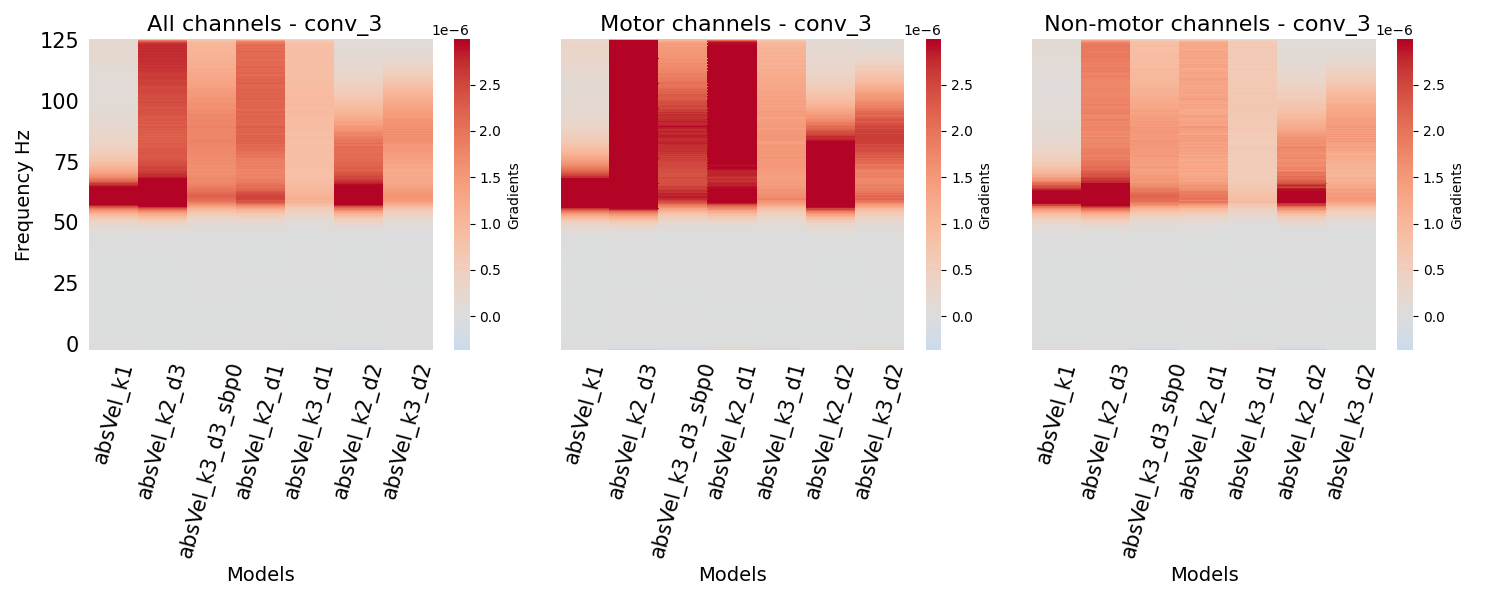
\includegraphics[width=1\linewidth]{img/ch4/absVel-conv-3-layer-grads-hp-shifted}
   \caption{}
\end{subfigure}\label{fig:absVel-conv-3-layer-grads-shifted-hp}
\caption[]{}
\end{figure}\label{fig:absVel-shifted-vs-non-shifted-grads-hp}

\subsubsection{Summary}\label{subsubsec:centre-shiftig-summary}
When looking at the performances and gradients of the various CNN architectures, the following observation can be made.
\begin{itemize}
    \item The shift improves performance 1. when training and validating on the full dataset; 2. when training on the full dataset and validating on low-passed data;
    3. when training and validating on high-passed data. This is true for both velocity and absolute velocity.
    \item The shift attenuates the differences in performance between the different CNNs for the full training and validation.
    When looking at graphs \textbf{B} in both~\cref{fig:shifted-performance-vel} and~\cref{fig:shifted-performance-absVel}, we can see that the number of network which have a significantly better performance than the original Deep4Net (k3\_d3\_sbp0) decreases compared to \textbf{A}.
    \item The shift does not improve performance for the CNNs trained on full data and validated on high-pass data (graphs \textbf{G} and \textbf{H} in both~\ref{fig:shifted-performance-vel} and~\ref{fig:shifted-performance-absVel}).
    This result together with the more narrow frequency bands the networks focus on after the shift show, that opposite to the expectation, the networks do not start focusing on high-gamma with the shift.
    They start to focus more on information from the lower frequency bands which.
    Modulations in these low frequency bands become more informative with the shift, therefore the performance increase, and the interest of the CNNs in higher frequencies drops.
    \item It is true in the shifted setting, as was in the non-shifted setting, that the network without max-pool (k1) which is most solely focused on low-frequency modulations performs the best.
    \item The modulations in the high-gamma band also become more informative for decoding with the shift, thus the increase in performance when training and validating on the high-passed dataset.
    Nevertheless, as we state in the point above, not even this motivates the networks to use information from the high-gamma band.
    The opposite happens.
\end{itemize}

From the observations above, we can state, that the modulations in the high-gamma band are not particularly informative for velocity and absolute velocity decoding.
They contain information the CNNs are able to use for decoding, nevertheless, it is not an advantage for the CNN, rather it harms its performance.
It is better for the CNNs to focus on low frequencies.


\subsection{Shifting the predicted time-point across receptive field}\label{subsec:shifting-the-predicted-time-point-across-receptive-field}
Besides the big shift from the edge of the receptive field to the centre we also studied what happens if we shift the predicted time-point in smaller steps across the receptive field of the network. 
The shifts are made ranging from  -1 s  to 1 s with respect to the receptive field centre which we denote as 0.
The step size was 0.1 s which is equivalent to 25 samples.
This way, we can observe how the shifting gradually influences the performance and gradients of the network. 

Unlike the previous experiments we chose to perform this analysis only on one architecture, namely, the Deep4Net\_sbp0. 
The shift seems to influence the gradients of all the networks similarly.
And therefore, the amount of time and computational power necessary to train multiple networks for each time-steps seems excessive.  

\subsubsection{Performance}\label{subsubsec:across-shiftig-performace}
The performance gradually changing with the shift is displayed in Figure~\ref{fig:shiftig-performance}.
We can observe the slow decrease in performance when increasing the distance of the predicted time-point to the receptive field centre, in both directions. 
This is to be expected. 
Nevertheless, similarly to performance in section~\ref{subsec:shifting-the-predicted-time-point-to-the-centre-of-the-receptive-field} we do not know if the fact that the performance peaks in the centre of the receptive field is due to the predicted time-point being in the centre of the receptive field.
It could again also be due to the fact that the network has information from the future. 
Interestingly, the decoding performance drops slower when using information predominantly from the future more than when using information predominantly from the past.
To properly investigate the informativeness of past vs. future signals however, we would need to have a network with an uniform receptive field. 
\todo{some literature about this}.

\begin{figure}[!hpbp]
\begin{subfigure}[a]{\textwidth}
   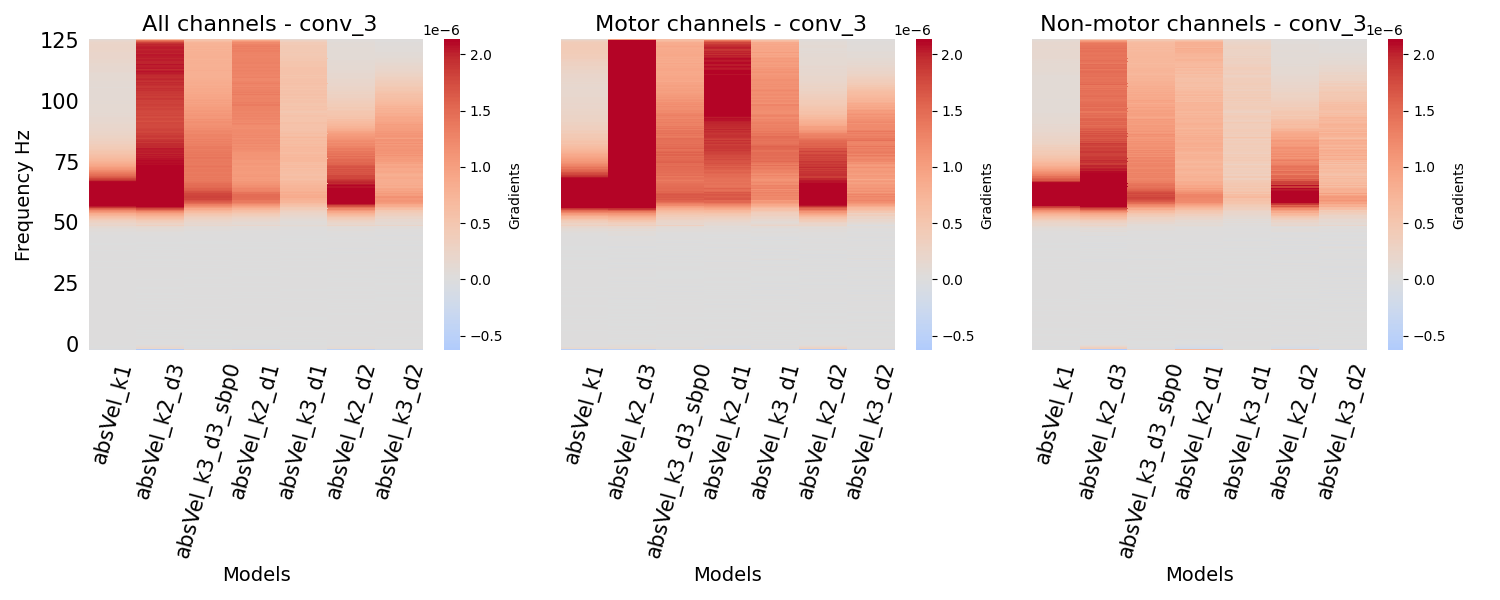
\includegraphics[width=1\linewidth]{img/ch4/absVel-conv-3-layer-grads-hp}
   \caption{}
\end{subfigure}\label{fig:vel-shifting-performance}

\begin{subfigure}[b]{\textwidth}
   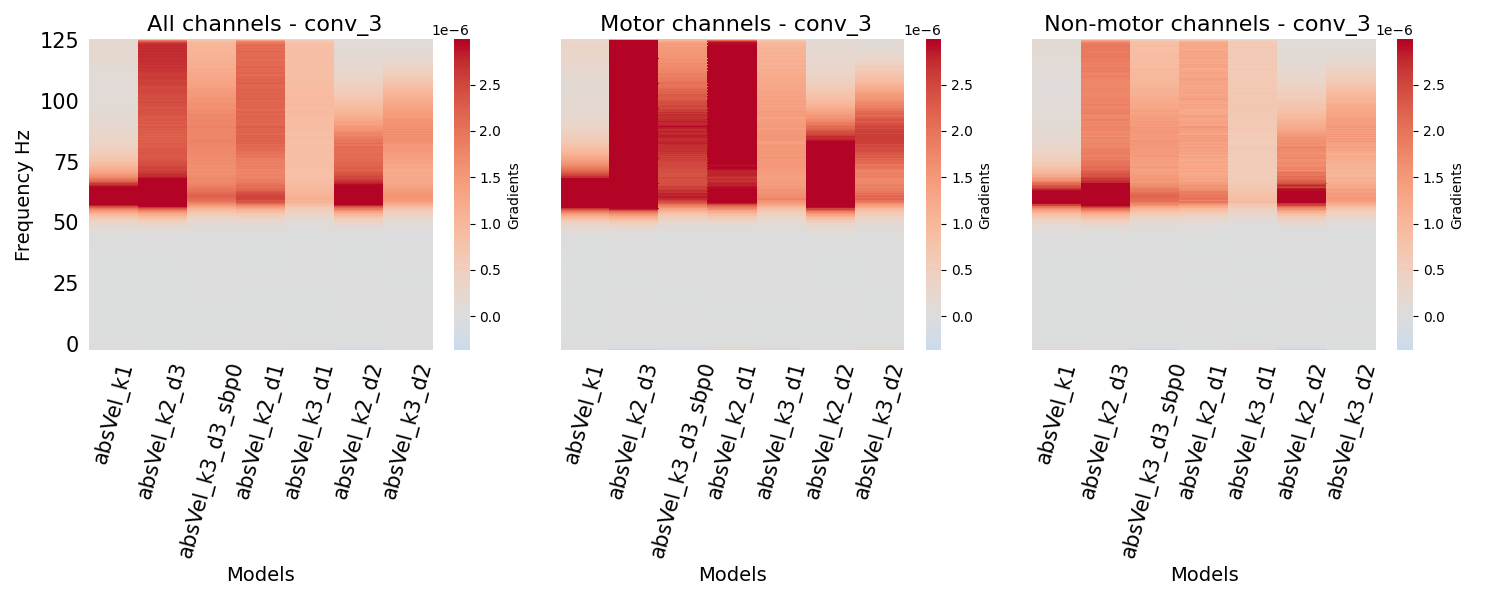
\includegraphics[width=1\linewidth]{img/ch4/absVel-conv-3-layer-grads-hp-shifted}
   \caption{}
\end{subfigure}\label{fig:absVel-shiftig-performance}
\caption[]{}
\end{figure}\label{fig:shifting-performance}

Besides observing how performance changes with shifting, we also visualize the gradients as is described in the next section.

\subsubsection{Gradients}\label{subsubsec:across-shiftig-gradients}
The gradients are visualized in Figure~\ref{figure-shifted-gradients}.
In the graph for absolute velocity, we can observe the trend of broadening the frequency ranges with high gradient values when shifting the predicted time-point from the centre of the receptive field both to the left and to the right.
This is what we expected because it corresponds to the results from~\cref{subsec:shifting-the-predicted-time-point-to-the-centre-of-the-receptive-field}.
Interestingly, when plotting the same graph for velocity, we do not observe this behaviour so clearly, instead there is a periodicity in the positive and negative value of the gradients for the different values of the shift.
It is unclear why this periodicity occurs.

\subsubsection{Summary}\label{subsubsec:across-shiftig-summary}
Besides the periodicity of the positive and negative values of the gradients in for velocity, we have further confirmed the conclusions we drew previously in \ref{subsec:shifting-the-predicted-time-point-to-the-centre-of-the-receptive-field}. 
Indeed the network seems to focus on more narrow frequency bands when given better access to information close to its receptive field.
In the case of the Deep4Net\_spb0 it also means lower interest in the high-gamma frequency band when achieving better performance.
This corroborates the what we have established so far about the information in the high-gamma band being inferior for velocity and absolute velocity decoding compared to information from lower frequency bands. 


\section{Spectral whitening}\label{sec:spectral-whitening}


\subsection{Performance}\label{subsec:pw-performance}
How the networks react to datasets which were whitened as described in Section~\ref{subsec:modifications-to-the-dataset} was one of our interests because when we look at the spectrum of the original signal, the amplitudes of frequencies decrease exponentially with increase in the frequency.
This is common in biological signals but could be a reason for the network to ignore high-frequencies when making predictions. Figure~\ref{pw-performances-full-data} shows how the predictions changed compared to predictions on non-whitened signals when using the full dataset.
It is obvious that the correlation coefficient of all networks dropped significantly.
When looking at Figure~\ref{pw-performaces-hp-data} we see that in the case of high-passed datasets the decrease was lower, but even for the high-passed data, the performance did not increase.

\subsection{Gradients}\label{subsec:pw-gradients2}

When looking at the gradients of the networks trained on whitened data, we observe that the networks indeed use modulations in the high-gamma frequency bands for their predictions.
Interestingly instead of having uniform gradients across all frequencies, they inverted their focus from low frequencies to high-frequencies.
The only architectures for which this did not happen are the models vel\_k1 and absVel\_k1 which are the networks without a max-pool layer.
When looking at the performance graphs in Figure~\ref{} though, these are the networks for which the performance dropped least.
This again suggests that the using information from the high-gamma frequency is possible, but it does not seem to help achieve better correlation coefficients.

\subsection{Summary}\label{subsec:pw-summary}